% Manual de Desarrollador
% Modificado por Crisostomo Barajas a partir del manual creado por Emmanuel Martinez
% Julio 2022

\documentclass[12pt,twoside,letter]{ol-softwaremanual}
\usepackage{float}
\usepackage[utf8]{inputenc}
\usepackage[a4paper,width=160mm,top=25mm,bottom=25mm]{geometry}
\usepackage[lining,tabular]{fbb} % so math uses tabular lining figures
\usepackage{graphicx}
\usepackage{enumitem}
\setlist{leftmargin=*}
\usepackage{listings}
\lstset{basicstyle=\ttfamily,frame=single,xleftmargin=3em,xrightmargin=3em}
\usepackage[os=win]{menukeys}
\renewmenumacro{\keys}[+]{shadowedroundedkeys}
\usepackage{framed}
\usepackage{etoolbox}
\AtBeginEnvironment{leftbar}{\sffamily\small}
\usepackage{array,lipsum}
\newenvironment{fulltable}[1][H]
 {\begin{table}[#1]%
  \hspace*{-\leftmarginwidth}%
  \begin{minipage}{\fullwidth}}
 {\end{minipage}\end{table}}
\usetikzlibrary{chains,arrows,shapes,positioning}
\usepackage{hyperref}
\graphicspath{{figures/}} %Setting the graphicspath
\renewcommand\abstractname{Introduction}

\usepackage[spanish]{babel}

\usepackage{multicol}

\usepackage{caption}
\usepackage[rightcaption]{sidecap}
\usepackage{subcaption}
\usepackage{wrapfig}
\usepackage{pifont}
\usepackage{fontawesome}

\usepackage{amsmath}
\usepackage{amssymb}

\usepackage{fancyhdr}

\pagestyle{fancy}
\fancyhf{}
\fancyhead[LE,RO]{{\footnotesize HDSP - UIS}}
\fancyhead[RE,LO]{{\footnotesize ReDs - Manual de Desarrollador}}
\fancyfoot[CE,CO]{\thepage}
%\fancyfoot[LE,RO]{\thepage}

\definecolor{ClearPurple}{RGB}{136, 0, 255}

\usepackage{tikz}
\newcommand*\circled[1]{\tikz[baseline=(char.base)]{
            \node[shape=circle,draw,inner sep=2pt] (char) {#1};}}

\newenvironment{Figure}
  {\par\medskip\noindent\minipage{\linewidth}}
  {\endminipage\par\medskip}
  
%\setlength{\parskip}{2em}
\setlength{\parskip}{6pt}%
\setlength{\parindent}{0pt}%
\setlength{\itemsep}{0em}

\title{\large{Manual de Desarrollo}\\ \vspace{10mm} \huge{Reconstrucción de Datos Sísmicos}\\ \vspace{5mm} \huge{ReDs}}
\author{
\includegraphics[width=14cm]{figures/all_logos3.png} \\ Emmanuel Martínez \\ Crisóstomo A. Barajas-Solano \\ Edwin Vargas}
\softwarelogo{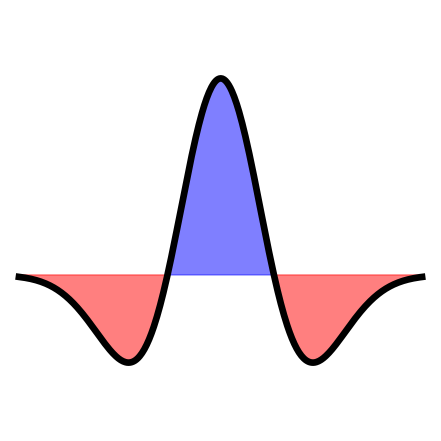
\includegraphics[width=7cm]{figures/icon}}
\version{2023.3}



\begin{document}

\maketitle

\newpage\null\thispagestyle{empty}\newpage

\begin{center}
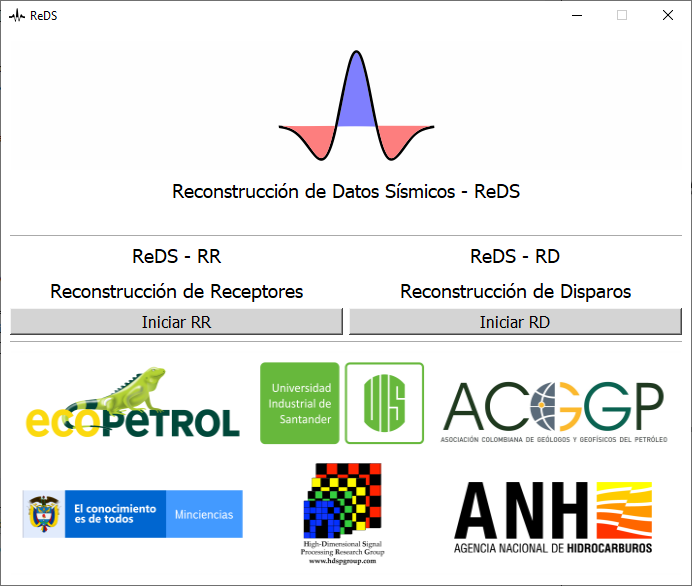
\includegraphics[width=.65\linewidth]{launch.png}
\end{center}
\begin{abstract}
%\includegraphics[width=1.0\linewidth]{PhysLogger.png}\\
%Esta aplicación pertenece al proyecto de investigación 9836, de la Universidad Industrial de Santander, Colombia. Esta aplicación permite la reconstrucción de trazas de muestras sísmicas mediante 4 diferentes algoritmos. Esta reconstrucción puede ser configurada por el usuario de tal manera que pueda realizar diferentes tipos de submuestreo y ajuste de parámetros mediante una interfaz gráfica de usuario.
La herramienta software Reconstrucción de Datos Sísmicos - ReDs hace parte del proyecto 9836 - ``Nuevas tecnologías computacionales para el diseño de sistemas de adquisición sísmica 3D terrestre con muestreo compresivo para la reducción de costos económicos e impactos ambientales en la exploración de hidrocarburos en cuencas terrestres colombianas''.

El proyecto 9836 está adscrito a la Convocatoria para la financiación de proyectos de investigación en geociencias para el sector de hidrocarburos, desarrollado por la alianza Universidad Industrial de Santander (UIS), ECOPETROL y la Asociación Colombiana de Geólogos y Geofísicos del Petróleo (ACGGP). 

Este proyecto es financiado por MINCIENCIAS y la Agencia Nacional de Hidrocarburos (ANH). Los derechos y licencias de uso sobre esta aplicación software están reservados a las entidades aportantes.
\end{abstract}

\newpage\null\thispagestyle{empty}\newpage

\clearpage
\tableofcontents

\clearpage

\newpage\null\thispagestyle{empty}\newpage

\section{Visión General de la Aplicación ReDs}

Esta aplicación Reconstrucción de Datos Sísmicos (ReDs) permite la reconstrucción de receptores y disparos sísmicos. Para esto, la aplicación ReDs dispone de dos modos de operación:
\begin{dingautolist}{192}
	\setlength\itemsep{0em}
	\item Reconstrucción de Receptores (ReDs - RR)
	\item Reconstrucción de Disparos (ReDs - RD)
\end{dingautolist}

\begin{Figure}
	\centering
	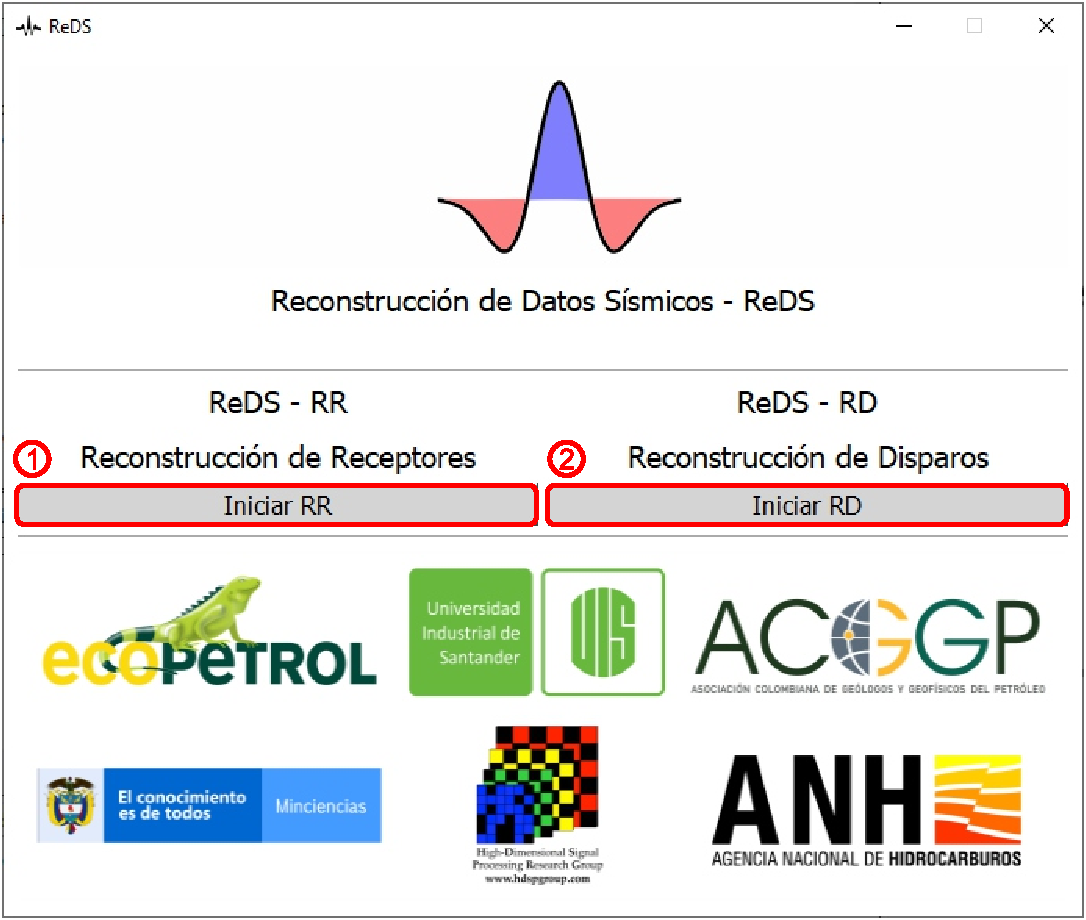
\includegraphics[width=0.65\linewidth]{launch2}
	\captionof{figure}{Secciones de la pantalla de inicio de ReDs.}
	\label{fig:launch}
\end{Figure}

Ambos modos de operación, RR y RD, realizan la reconstrucción de datos sísmicos usando 4 algoritmos numéricos diferentes:
\begin{itemize}[leftmargin=0.5in]
	\setlength\itemsep{0em}
	\item FISTA (Fast Iterative Shrinkage-Thresholding Algorithm): permite resolver problemas inversos lineales mediante un algoritmo iterativo rápido
	\item GAP (Generalized Alternating Projection): resuelve el problema de seguimiento de base grupal, que extiende el seguimiento de base reemplazando la norma $ \ell_1 $ por una norma ponderada $ \ell_{2,1} $.
	\item TwIST (Two-step Iterative Shrinkage/Thresholding): basado en el algoritmo ISTA, permite la resolución de problemas inversos
	\item ADMM (Alternating Direction Method of Multipliers): resuelve problemas de optimización convexos dividiéndolos en partes más pequeñas.
\end{itemize}

El usuario puede configurar cada uno de los algoritmos de reconstrucción de tal manera que pueda realizar diferentes tipos de submuestreo y ajuste de parámetros, todo desde una interfaz gráfica de usuario simple y clara. Aunque los modos de reconstrucción RR y RD presentan diferencias en su operación, están diseñados bajo las mismas directivas. Por esta razón, ambas interfaces gráficas cuentan con varias secciones en común.



\cleardoublepage

\section{Módulo ReDs - Reconstrucción de Receptores (RR)}

El módulo ReDS-RR (reconstrucción de receptores) realiza la estimación de trazas faltantes en un disparo sísmico, usando algoritmos de gradiente descendiente y aprovechando representaciones escasas de los datos en dominios transformados como Curvelet, DCT y Wavelets.

A continuación se mostrará de forma especifican los modos de uso del módulo ReDs - RR, las diferentes configuraciones y opciones que pueden ser aplicadas a los datos sísmicos para la realización de diferentes tipos de experimentos. Cabe resaltar que de acuerdo al tipo de prueba que se quiera realizar, el comportamiento de los paneles cambiará para adecuarse a dicha tarea.

\subsection{Requerimientos}

La aplicación ReDs - RR cuenta con una barra de tareas en la parte superior de la ventana. Aquí se observan 3 botones distintos que permitirán realizar distintos tipos de pruebas sobre los datos sísmicos.

\begin{multicols}{2}
	
	Como se observa en la figura \ref{fig:main_button}, el primer botón habilitará a el Modo Sencillo para realizar pruebas generales sobre los datos sísmicos.
	
	La figura \ref{fig:vision} presenta las 7 secciones de la interfaz general del Modo Sencillo de ReDs - RR, a mencionar:
	
	\begin{Figure}
		\centering
		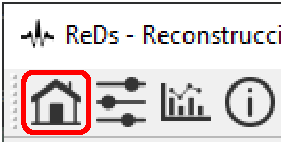
\includegraphics[width=0.5\linewidth]{single-tab}
		\captionof{figure}{Botón del menú principal.}
		\label{fig:main_button}
	\end{Figure}
	
\end{multicols}


\begin{dingautolist}{192}
	\setlength\itemsep{0em}
	\item Barra del menú
	\item Lector de datos
	\item Panel de algoritmos
	\item Panel de submuestreo
	\item Menú de experimentos
	\item Menú de cambio de vista
	\item Menú de visualización
\end{dingautolist}

\begin{Figure}
	\centering
	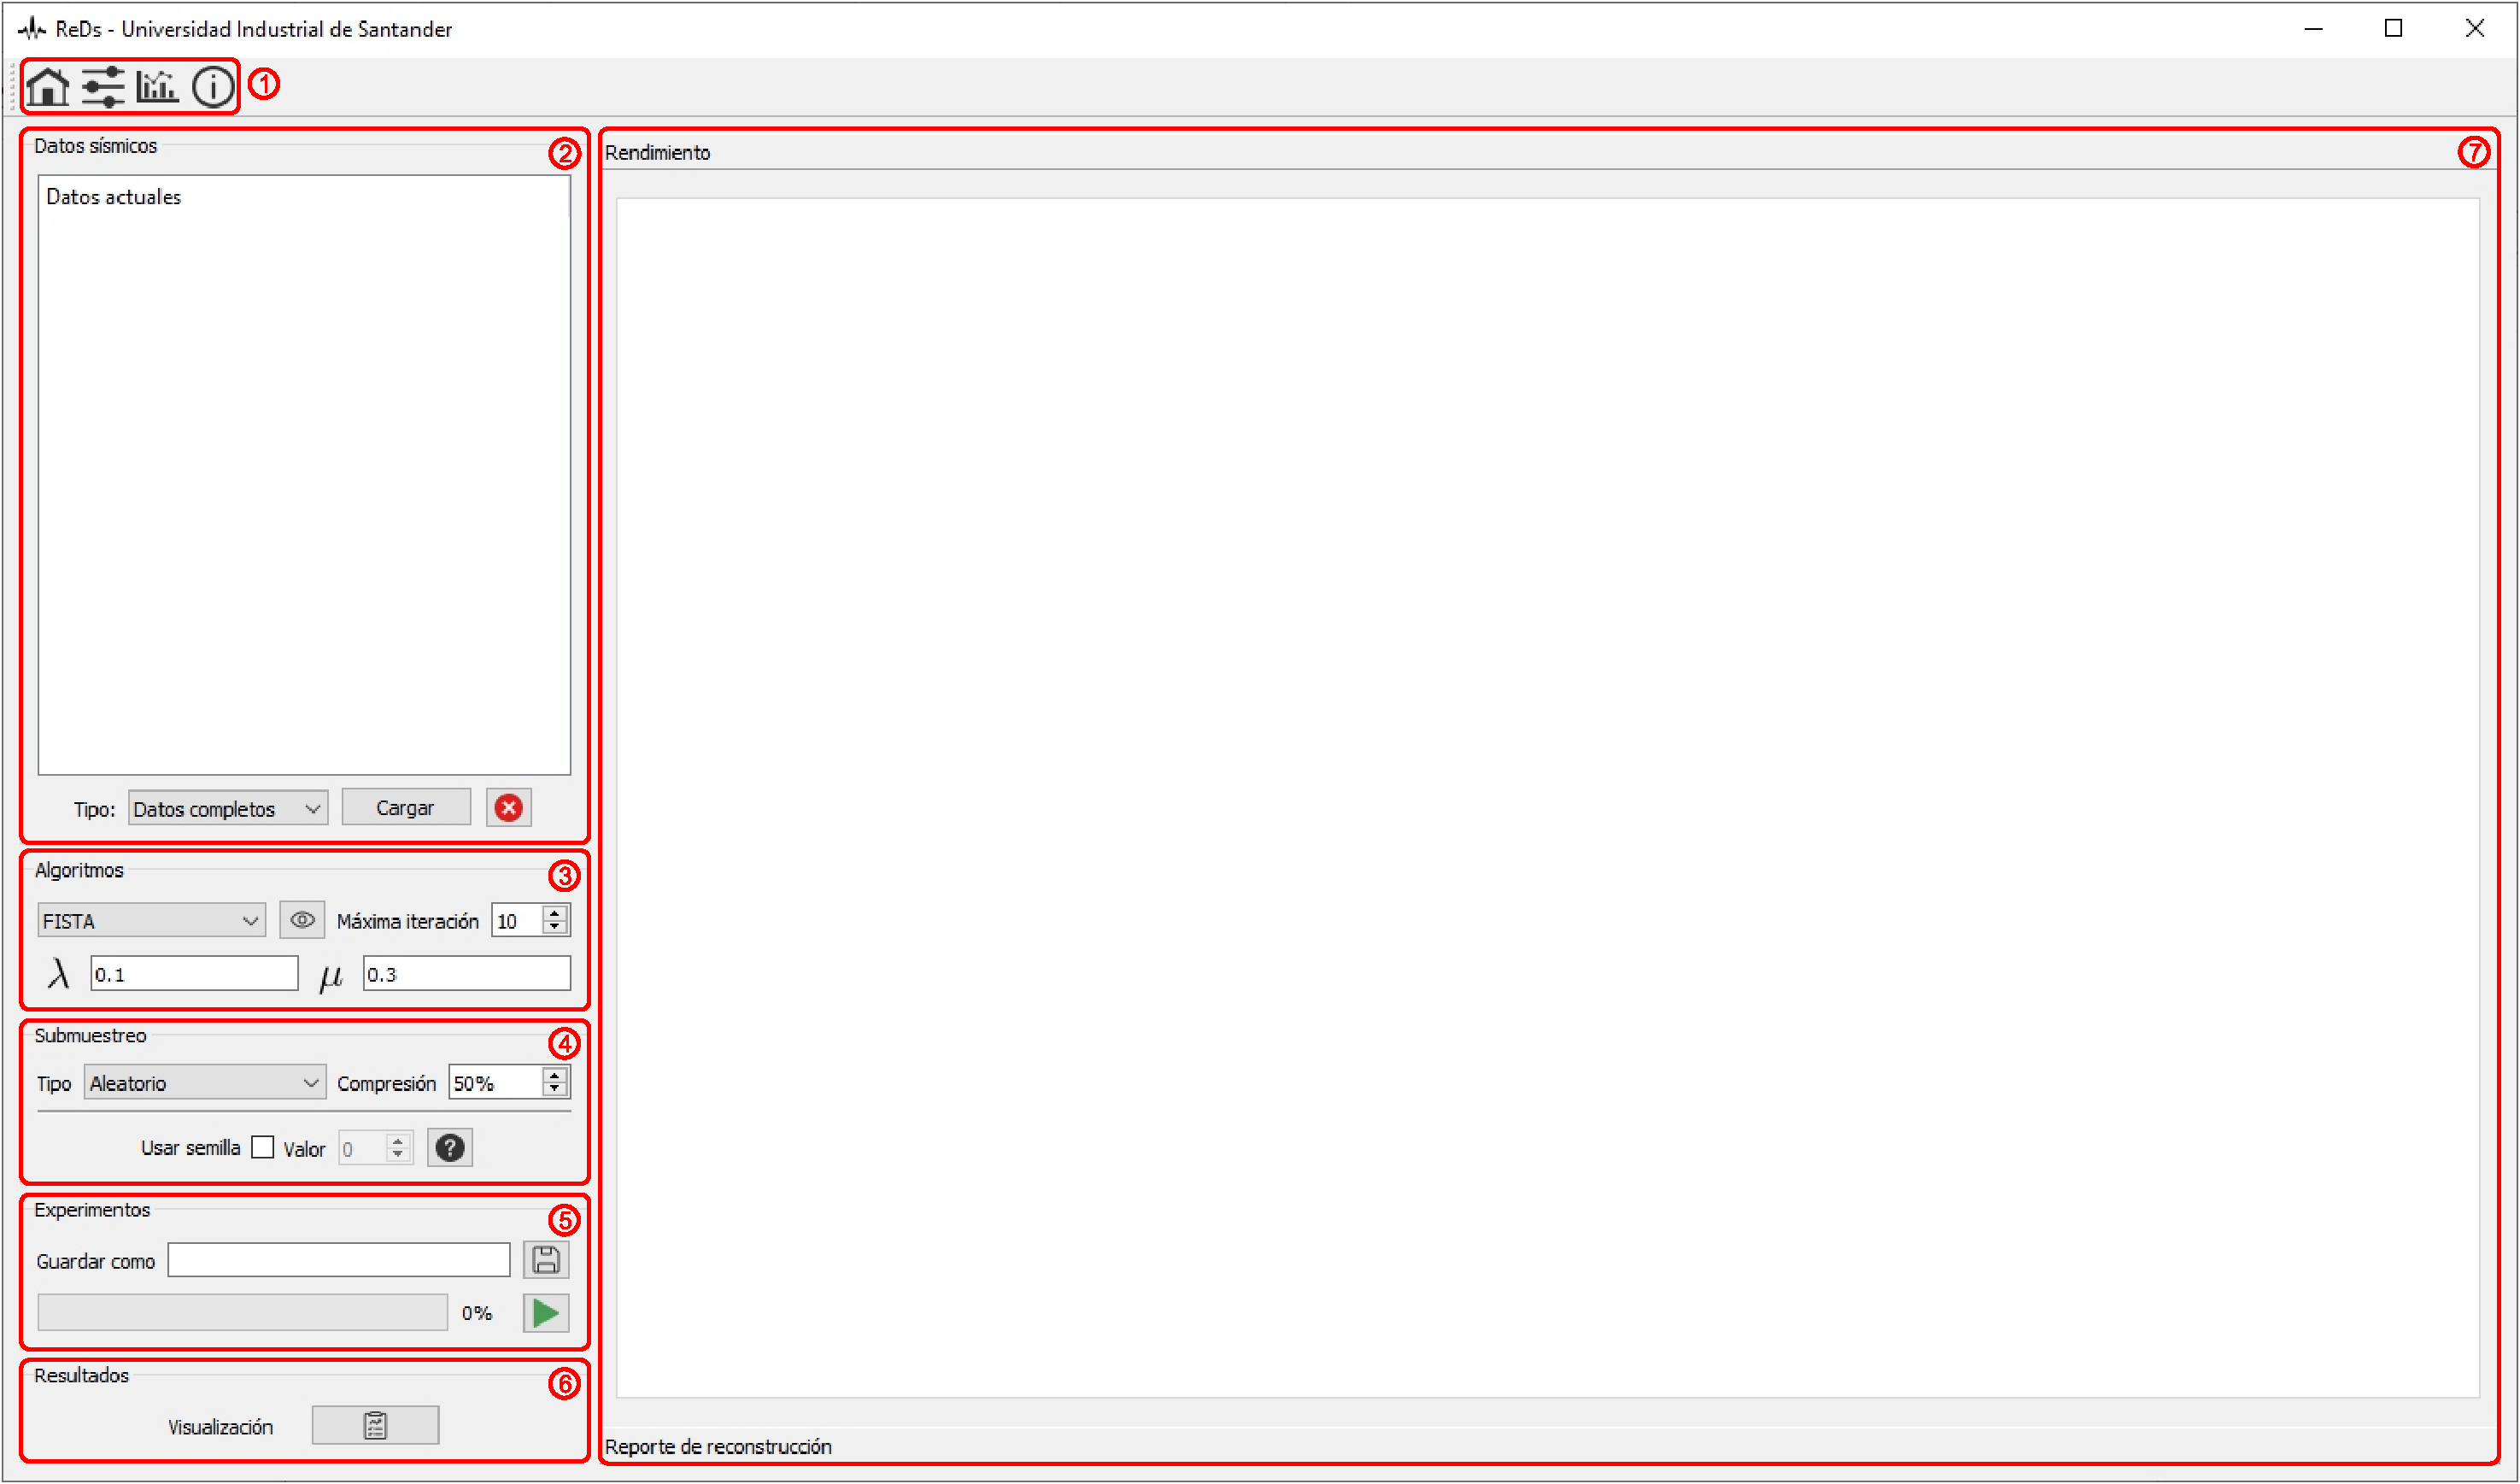
\includegraphics[width=1\linewidth]{figures/vision_v2}
	\captionof{figure}{Secciones de la interfaz general del modo Reds - RR.}
	\label{fig:vision}
\end{Figure}



El menú principal permite realizar experimentos con los datos sísmicos siguiendo el orden que se observa en la figura \ref{fig:vision}. A continuación se muestra paso a paso el funcionamiento de cada uno los paneles, desde la lectura de datos sísmicos hasta la visualización y guardado de resultados.

\subsection{Políticas de diseño}

El panel de lectura de datos \circled{2}, situado al extremo izquierdo superior en la figura \ref{fig:vision}, muestra los nombres de los datos sísmicos que el usuario haya cargado en la aplicación para realizar diversas pruebas.\\

\textbf{Leyendo un dato sísmico} \label{sec:data_lecture}

\begin{multicols}{2}
	
\begin{Figure}
	\centering
	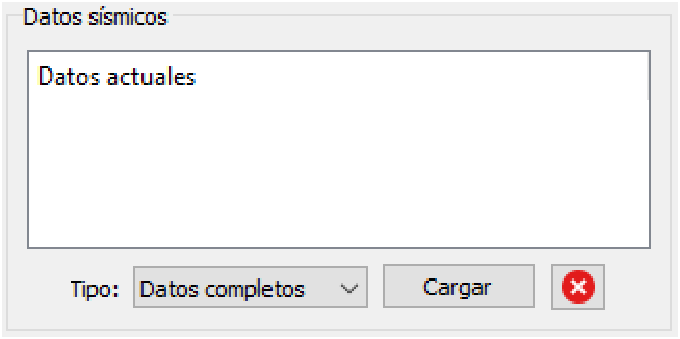
\includegraphics[width=.9\linewidth]{data-lecture-1.pdf}
	\captionof{figure}{Cargando un dato sísmico.}
	\label{fig:data_lecture_1}
\end{Figure}

Para leer un dato sísmico, se pulsa la opción \emph{Cargar} en el panel \circled{2}, como se observa en la figura \ref{fig:data_lecture_1}. Inmediatamente se abrirá la ventana \textit{Abrir dato sísmico}, como se observa en la figura \ref{fig:data_lecture_2}, donde el usuario podrá seleccionar un dato sísmico. Para este ejemplo cargaremos \emph{data.npy}.
La aplicación ReDs reconoce las extensiones \emph{.npy} y \emph{.mat} para cargar datos sísmicos.

\end{multicols}

Existen dos tipos de datos sísmicos que pueden ser cargados desde ReDs - RR: \textit{Datos Completos} y \textit{Datos Incompletos}. El tipo de dato a ser cargado puede ser seleccionado desde la lista desplegable en la Figura \ref{fig:data_lecture_1}.

\begin{Figure}
    \centering
    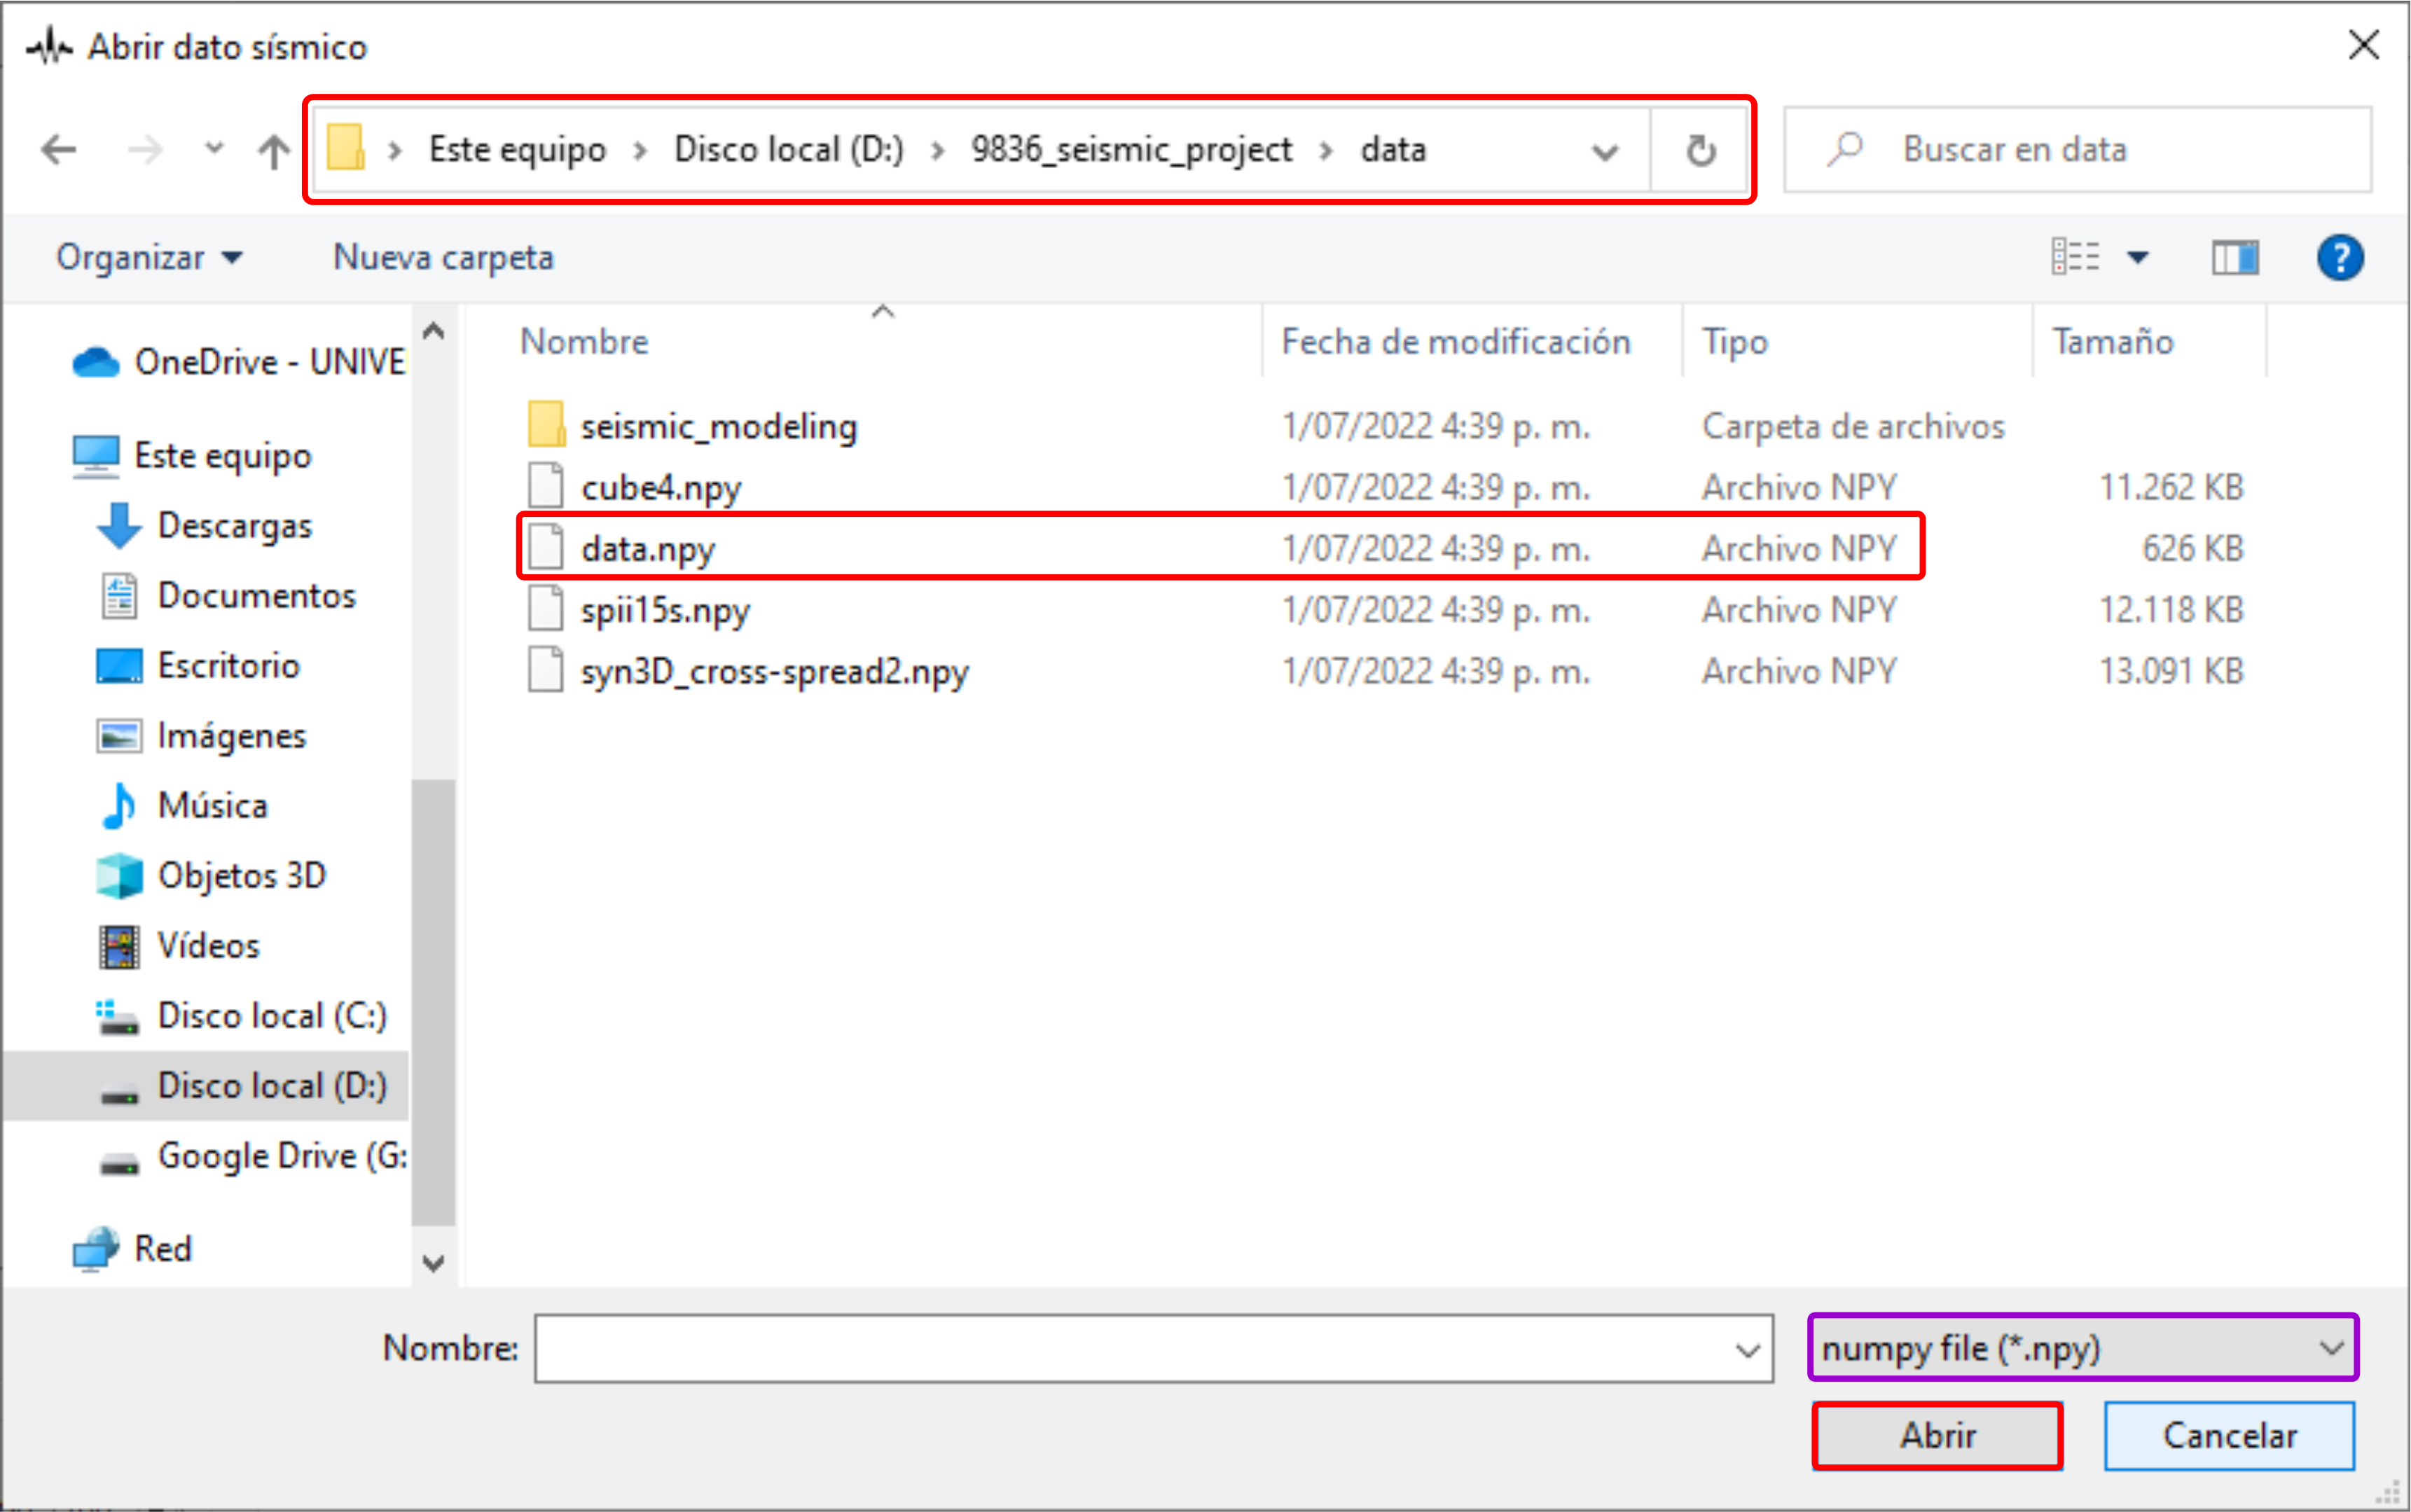
\includegraphics[width=1\linewidth]{data-lecture-2.png}
     \captionof{figure}{Ventana de selección de dato sísmico.}
    \label{fig:data_lecture_2}
\end{Figure}

\begin{multicols}{2}

Una vez seleccionado el dato sísmico, se debe pulsar en la opción \emph{Abrir}. Se podrá observar entonces en \circled{2} el dato sísmico cargado, como se muestra en la figura \ref{fig:data_lecture_3}. Aquí los datos se observan siguiendo la siguiente estructura: \circled{I} representa al directorio padre y \circled{II} es el dato sísmico cargado hijo del directorio padre.

\begin{Figure}
    \centering
    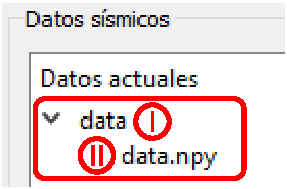
\includegraphics[width=0.6\linewidth]{data-lecture-3.pdf}
     \captionof{figure}{Panel con un dato sísmico cargado.}
    \label{fig:data_lecture_3}
\end{Figure}

\end{multicols}

\subsection{Diagramas UML}

Los algoritmos disponibles en la aplicación son \emph{FISTA}, \emph{GAP}, \emph{TwIST} y \emph{ADMM}, tal como se observa en el panel \circled{3}, en el extremo izquierdo de la figura \ref{fig:vision}. En este panel se pueden observar las opciones de configuración de parámetros según el algoritmo seleccionado, incluyendo la cantidad máxima de iteraciones a realizar. 

\begin{figure}[!ht]
     \centering
     \begin{subfigure}[b]{0.47\textwidth}
         \centering
         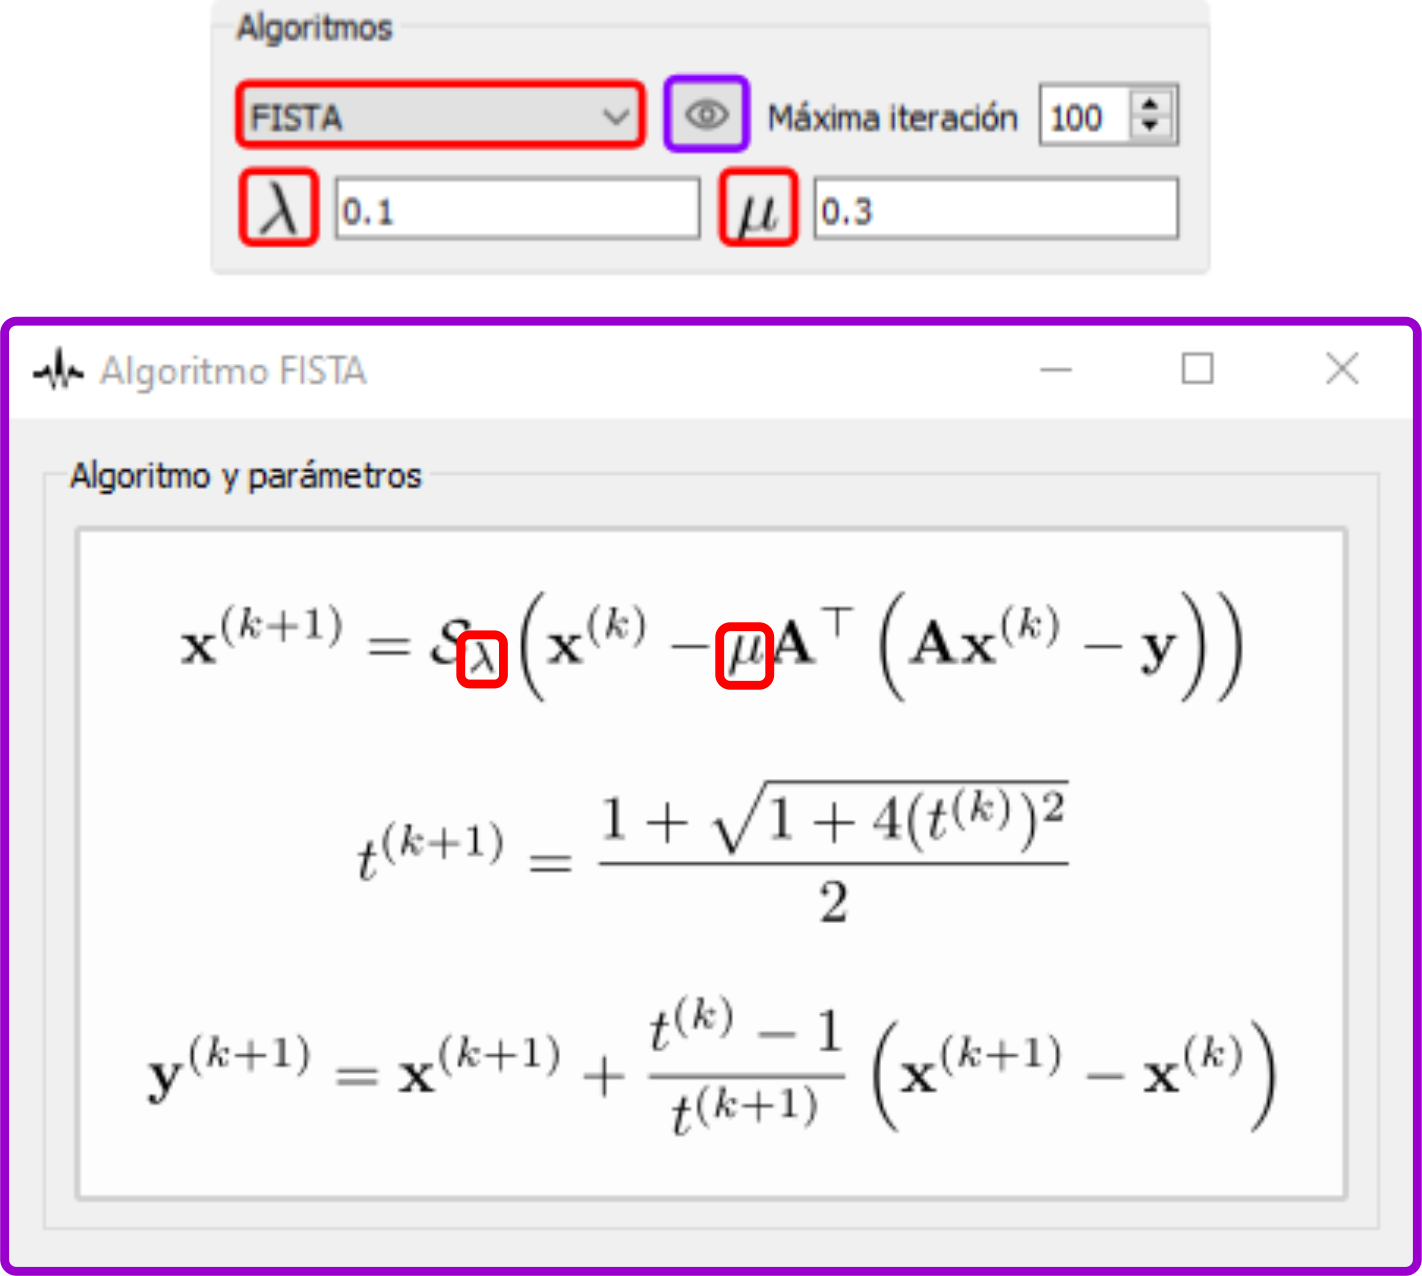
\includegraphics[width=\textwidth]{algorithm-fista.png}
         \caption{FISTA}
         \label{fig:fista}
     \end{subfigure}
     \hfill
     \begin{subfigure}[b]{0.47\textwidth}
         \centering
         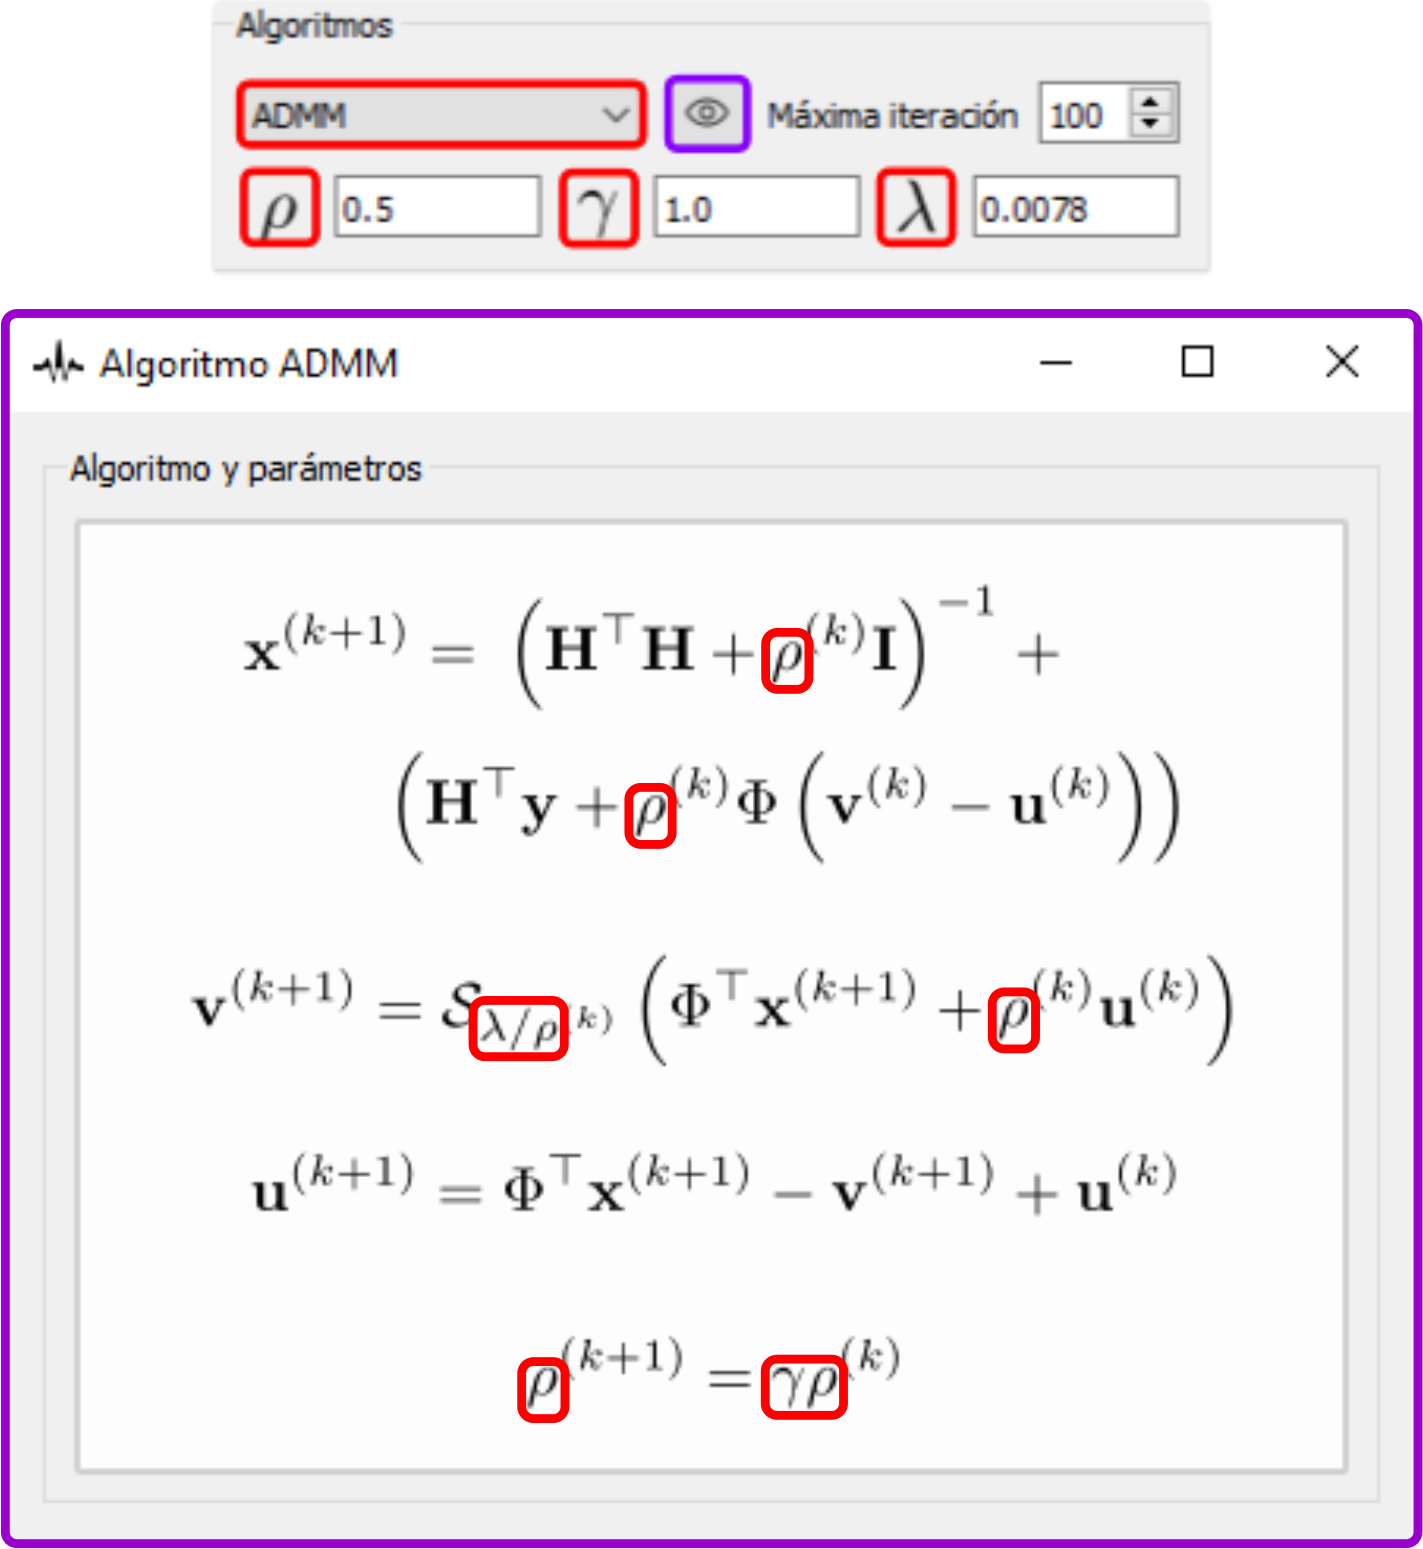
\includegraphics[width=\textwidth]{algorithm-admm.png}
         \caption{ADMM}
         \label{fig:admm}
     \end{subfigure}
     \begin{subfigure}[b]{0.47\textwidth}
         \centering
         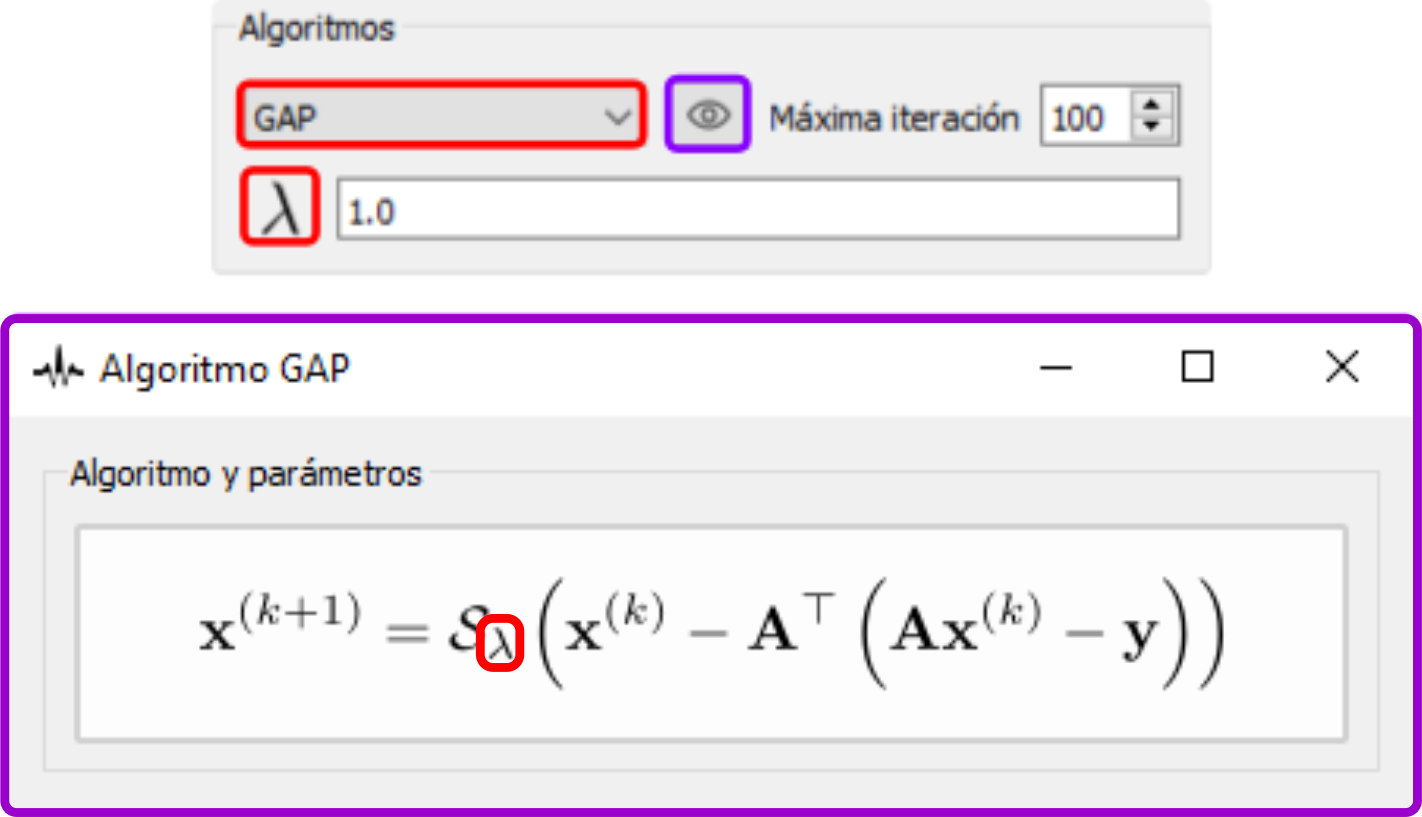
\includegraphics[width=\textwidth]{algorithm-gap.png}
         \caption{GAP}
         \label{fig:gap}
     \end{subfigure}
     \hfill
     \begin{subfigure}[b]{0.47\textwidth}
         \centering
         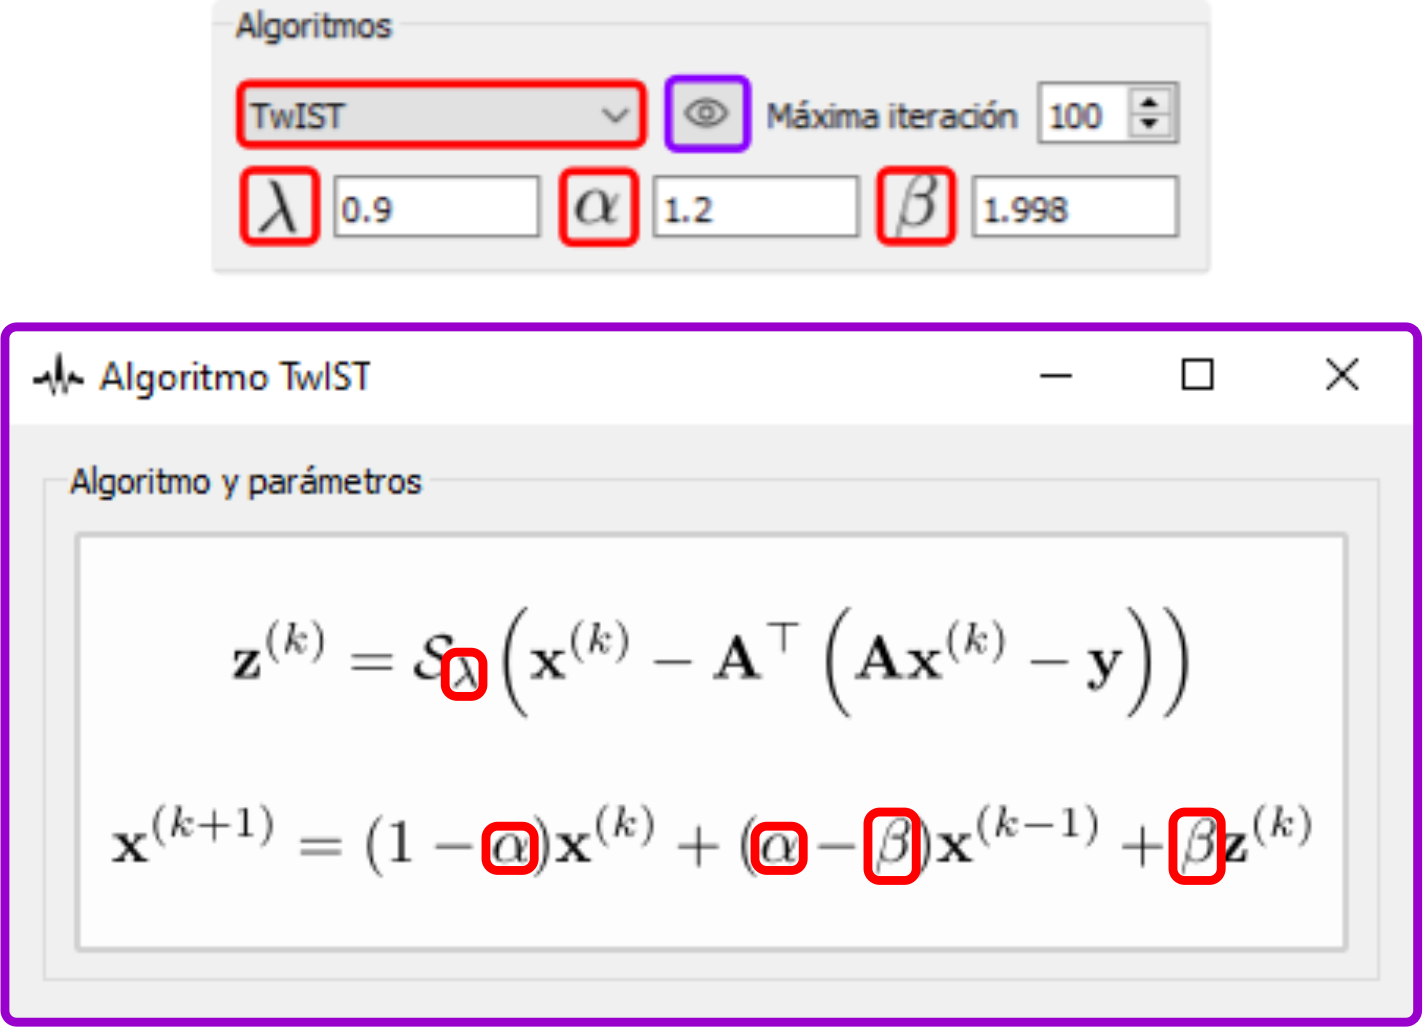
\includegraphics[width=\textwidth]{algorithm-twist.png}
         \caption{TwIST}
         \label{fig:twist}
     \end{subfigure}
        \caption{Algoritmos disponibles y sus respectivos parámetros.}
        \label{fig:algorithms}
\end{figure}

Adicionalmente, el botón\hspace{0.5mm} \faEye \hspace{0.5mm} permite visualizar los diferentes algoritmos con sus correspondientes parámetros, como se observa en la figura \ref{fig:algorithms}. Cada uno de los algoritmos disponibles cuenta con una colección propia de parámetros, los cuales el pueden ser configurados por el usuario según lo desee.

\subsubsection{Diagramas de casos de uso}\label{subsampling}

Debido a que hay varias formas de recuperar una traza a partir de las medidas recolectadas previamente, el panel de submuestreo \circled{4} permite configurar cuál tipo de submuestreo se desea realizar al dato sísmico, a manera de simulación. Todos los tipos de submuestreo, excepto el de tipo lista, comparten el mismo nivel de compresión que el usuario desee asignar. Por otra parte, al cargar datos incompletos el panel de submuestreo se deshabilita.

A continuación se presentan los tipos de submuestreo a aplicar en ReDs:\\

\underline{\textbf{Submuestreo Aleatorio}}

\begin{multicols}{2}
\begin{Figure}
	\centering
	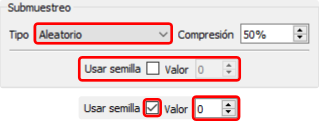
\includegraphics[width=0.8\linewidth]{subsampling-random.png}
	\captionof{figure}{Submuestreo aleatorio.}
	\label{fig:subsampling_random}
\end{Figure}

Aplica un submuestreo aleatorio a las trazas sísmicas de acuerdo al nivel de compresión. Al habilitar la semilla, se puede establecer el mismo submuestreo para todas las veces que se ejecute un experimento, como se observa en la figura \ref{fig:subsampling_random}.

\end{multicols}

\underline{\textbf{Submuestreo Uniforme}}

\begin{multicols}{2}

Aplica un submuestreo uniforme a las trazas sísmicas de acuerdo al nivel de compresión, como se observa en la figura \ref{fig:subsampling_uniform}.

\begin{Figure}
    \centering
    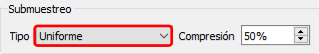
\includegraphics[width=0.8\linewidth]{subsampling-uniform.png}
     \captionof{figure}{Submuestreo uniforme.}
    \label{fig:subsampling_uniform}
\end{Figure}

\end{multicols}

\underline{\textbf{Submuestreo Jitter}}

\begin{multicols}{2}

\begin{Figure}
	\centering
	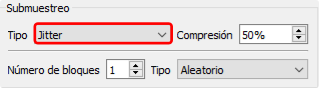
\includegraphics[width=0.8\linewidth]{subsampling-jitter.png}
	\captionof{figure}{Submuestreo jitter.}
	\label{fig:subsampling_jitter}
\end{Figure}

Aplica un submuestreo aleatorio o uniforme de acuerdo a la cantidad de bloques ingresados por el usuario a las trazas sísmicas de acuerdo al nivel de compresión, como se observa en la figura \ref{fig:subsampling_jitter}.

\end{multicols}

\underline{\textbf{Submuestreo Lista}}

\begin{multicols}{2}

Aplica un submuestreo de tipo lista donde las trazas a remover son ingresados por el usuario, como se observa en la figura \ref{fig:subsampling_list}. Para este tipo de submuestreo es necesario validar que el usuario ingrese los datos con un formato lógico y especifico.

\begin{Figure}
    \vspace{5mm}
    \centering
    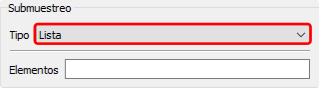
\includegraphics[width=0.8\linewidth]{subsampling-list.png}
     \captionof{figure}{Submuestreo de tipo lista.}
    \label{fig:subsampling_list}
\end{Figure}

\end{multicols}

Las condiciones son las siguientes:

\begin{multicols}{2}

\begin{Figure}
	\vspace{5mm}
	\centering
	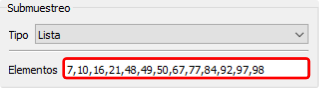
\includegraphics[width=1\linewidth]{subsampling-list-1.png}
	\captionof{figure}{Ejemplo de submuestreo de tipo lista.}
	\label{fig:subsampling_list_1}
\end{Figure}

\begin{itemize}
	\setlength\itemsep{0em}
    \item La secuencia debe ser $x_1,x_2,x_n$, tal que $x_i \in \mathbb{Z}^+$ representa los índices de las trazas a resolver, donde entre cada $x_i$ no deben haber espacios y estar separados por números, como se observa en la figura \ref{fig:subsampling_list_1}.
    \item Cada $x_i$ debe cumplir $0 \leq x_i \leq N$, donde $N$ es la cantidad máxima lineas de receptores que contiene un \emph{shot}.
    \item Deben haber mínimo siete $x_i$ distintos.
\end{itemize}

\end{multicols}

\subsubsection{Diagramas de casos de Secuencias}
\label{sec:experiment}

Una vez ya se ha cargado un dato sísmico, seleccionado el algoritmo, ajustado sus parámetros y configurado el tipo de submuestreo, entonces se podrá realizar un experimento. El panel \circled{5}, en el extremo izquierdo de la figura \ref{fig:vision}, permite controlar el progreso de la ejecución del experimento a realizar.
\newpage
\subsubsection*{Realizando un experimento}

\begin{multicols}{2}

Para iniciar un nuevo experimento se debe pulsar el botón \hspace{0.5mm} \faSave \hspace{0.5mm} que se observa en la figura \ref{fig:experiment_1}. Aquí el usuario seleccionará el directorio donde desee que los resultados de su experimento sean guardados, como se observa en la figura \ref{fig:experiment_2}.

\begin{Figure}
    \vspace{5mm}
    \centering
    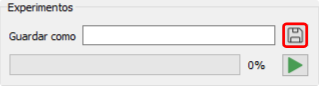
\includegraphics[width=0.8\linewidth]{experiment-1.png}
     \captionof{figure}{Panel de experimentos.}
    \label{fig:experiment_1}
\end{Figure}

\end{multicols}

\begin{Figure}
    \centering
    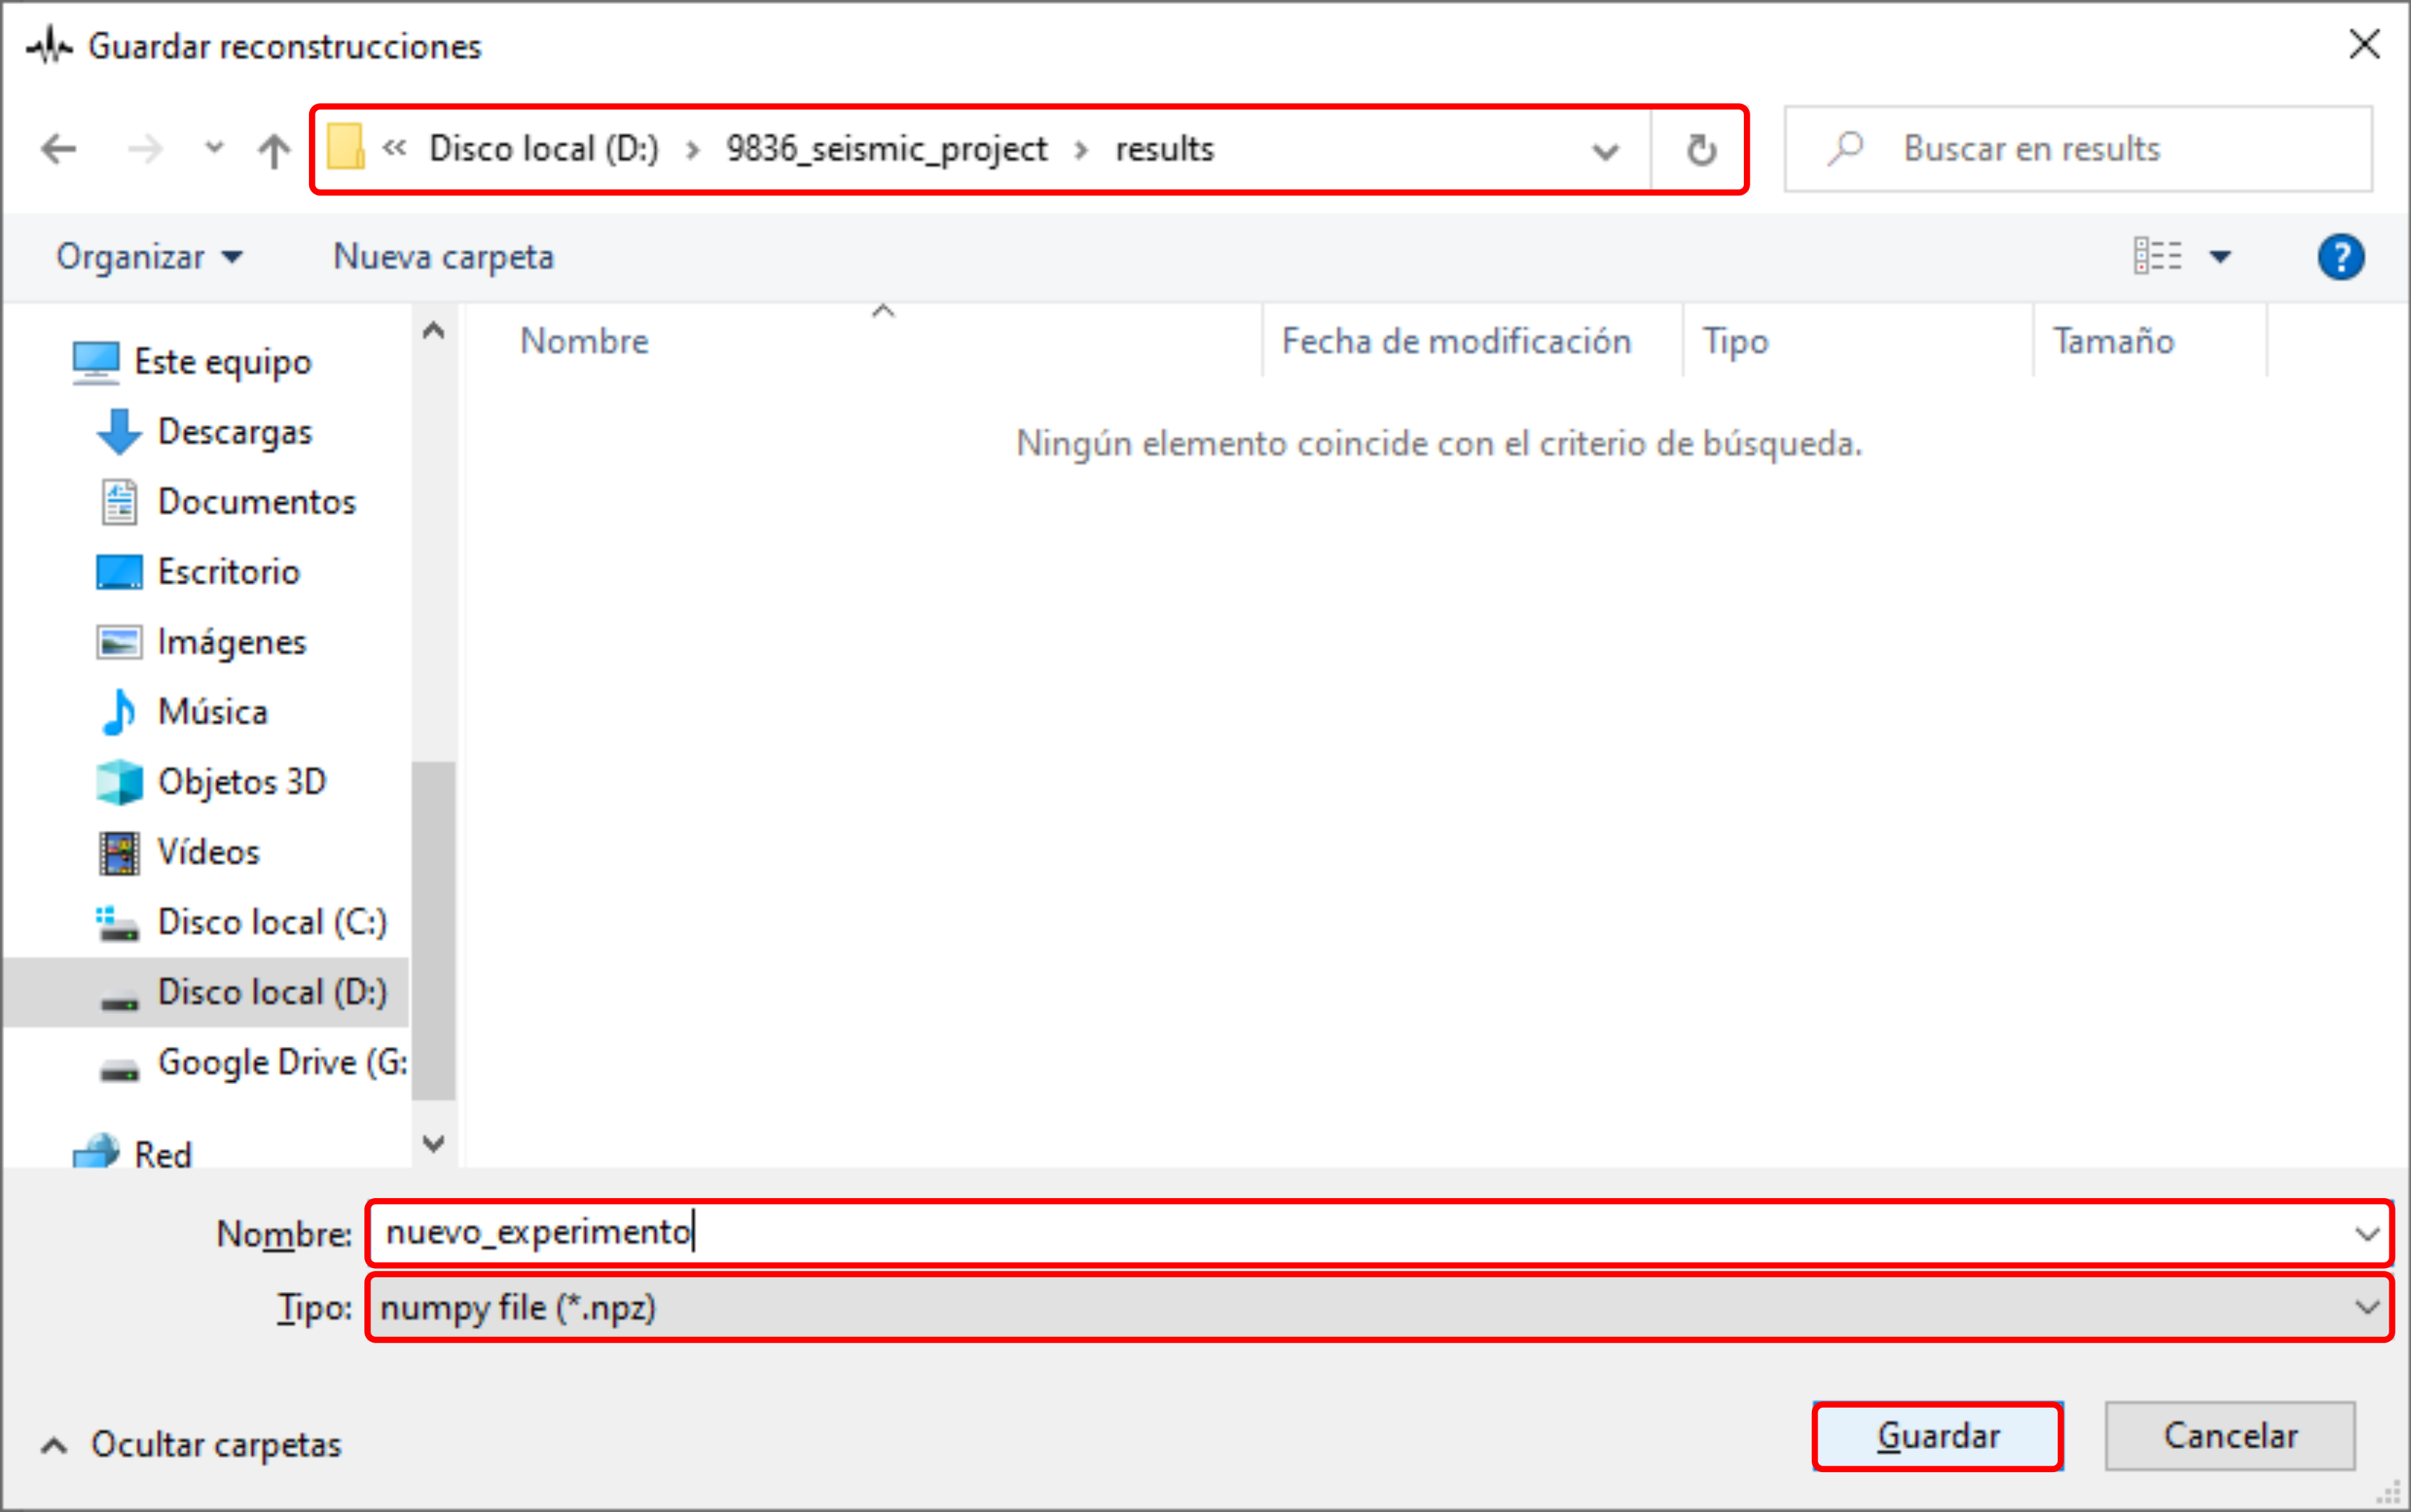
\includegraphics[width=1\linewidth]{experiment-2.png}
     \captionof{figure}{Ventana de guardado de resultados.}
    \label{fig:experiment_2}
\end{Figure}

Es necesario asignar un nombre al experimento para poder guardarlo. En este ejemplo usaremos \emph{nuevo\_experimento} como nombre del archivo de salida, con la extensión \emph{.npz}. Finalmente, presionamos el botón \emph{Guardar}.

\begin{multicols}{2}

\begin{Figure}
	\centering
	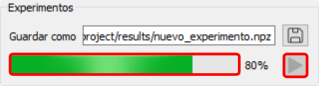
\includegraphics[width=0.7\linewidth]{experiment-4.png}
	\captionof{figure}{Ejecución de un experimento en tiempo real.}
	\label{fig:experiment_4}
\end{Figure}

Para correr el experimento se debe pulsar en el botón \hspace{0.5mm} \faPlay \hspace{0.5mm}. En la barra de progreso, a la izquierda de dicho botón, se podrá el progreso del actual experimento, como se observa en la figura \ref{fig:experiment_4}.

\end{multicols}

\subsubsection{Diagramas de Componentes}

Los resultados de todos los experimentos se pueden observar en el panel \circled{7}, en el extremo derecho de la figura \ref{fig:vision}. En este panel se encuentran dos tipos de visualización: la visualización del rendimiento (iteraciones vs. error/psnr) y visualización de la reconstrucción, como se observa en la figura \ref{fig:main_result_1}.

\begin{multicols}{2}

Como se mencionó en la sección \ref{sec:experiment}, para los experimentos que sean ejecutados se podrá ver tanto el rendimiento como la reconstrucción de las trazas en tiempo real. A continuación se detallará que es lo que se observa exactamente en cada una de estos subpaneles.

\begin{Figure}
    %\vspace{1cm}
    \centering
    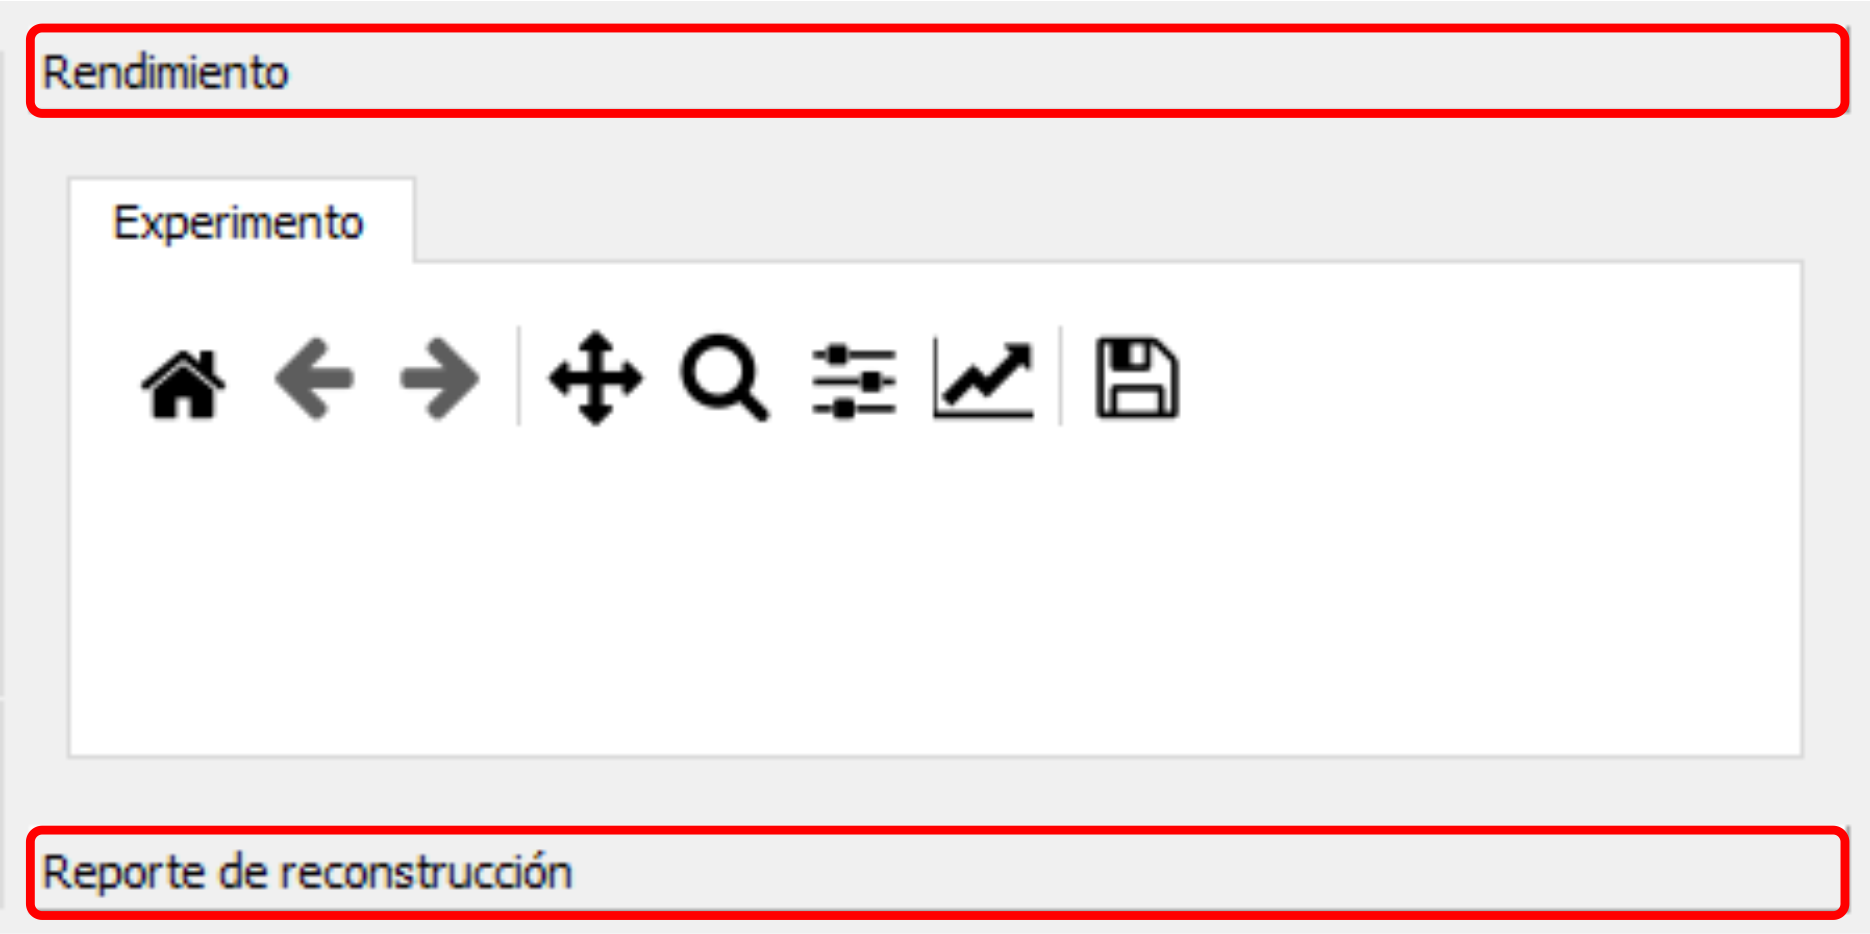
\includegraphics[width=0.7\linewidth]{main-result-1.png}
     \captionof{figure}{Panel de resultados.}
    \label{fig:main_result_1}
\end{Figure}

\end{multicols}

\subsubsection{Diagramas de Clases}
\newpage

\section{Módulo ReDs - Reconstrucción de Disparos (RD)}

El módulo ReDS-RR (reconstrucción de receptores) realiza la estimación de trazas faltantes en un disparo sísmico, usando algoritmos de gradiente descendiente y aprovechando representaciones escasas de los datos en dominios transformados como Curvelet, DCT y Wavelets.

A continuación se mostrará de forma especifican los modos de uso del módulo ReDs - RR, las diferentes configuraciones y opciones que pueden ser aplicadas a los datos sísmicos para la realización de diferentes tipos de experimentos. Cabe resaltar que de acuerdo al tipo de prueba que se quiera realizar, el comportamiento de los paneles cambiará para adecuarse a dicha tarea.

\subsection{Requerimientos}

La aplicación ReDs - RR cuenta con una barra de tareas en la parte superior de la ventana. Aquí se observan 3 botones distintos que permitirán realizar distintos tipos de pruebas sobre los datos sísmicos.

\begin{multicols}{2}
	
	Como se observa en la figura , el primer botón habilitará a el Modo Sencillo para realizar pruebas generales sobre los datos sísmicos.
	
	La figura  presenta las 7 secciones de la interfaz general del Modo Sencillo de ReDs - RR, a mencionar:
	
	\begin{Figure}
		\centering
		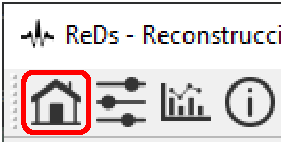
\includegraphics[width=0.5\linewidth]{single-tab}
		\captionof{figure}{Botón del menú principal.}
		
	\end{Figure}
	
\end{multicols}


\begin{dingautolist}{192}
	\setlength\itemsep{0em}
	\item Barra del menú
	\item Lector de datos
	\item Panel de algoritmos
	\item Panel de submuestreo
	\item Menú de experimentos
	\item Menú de cambio de vista
	\item Menú de visualización
\end{dingautolist}

\begin{Figure}
	\centering
	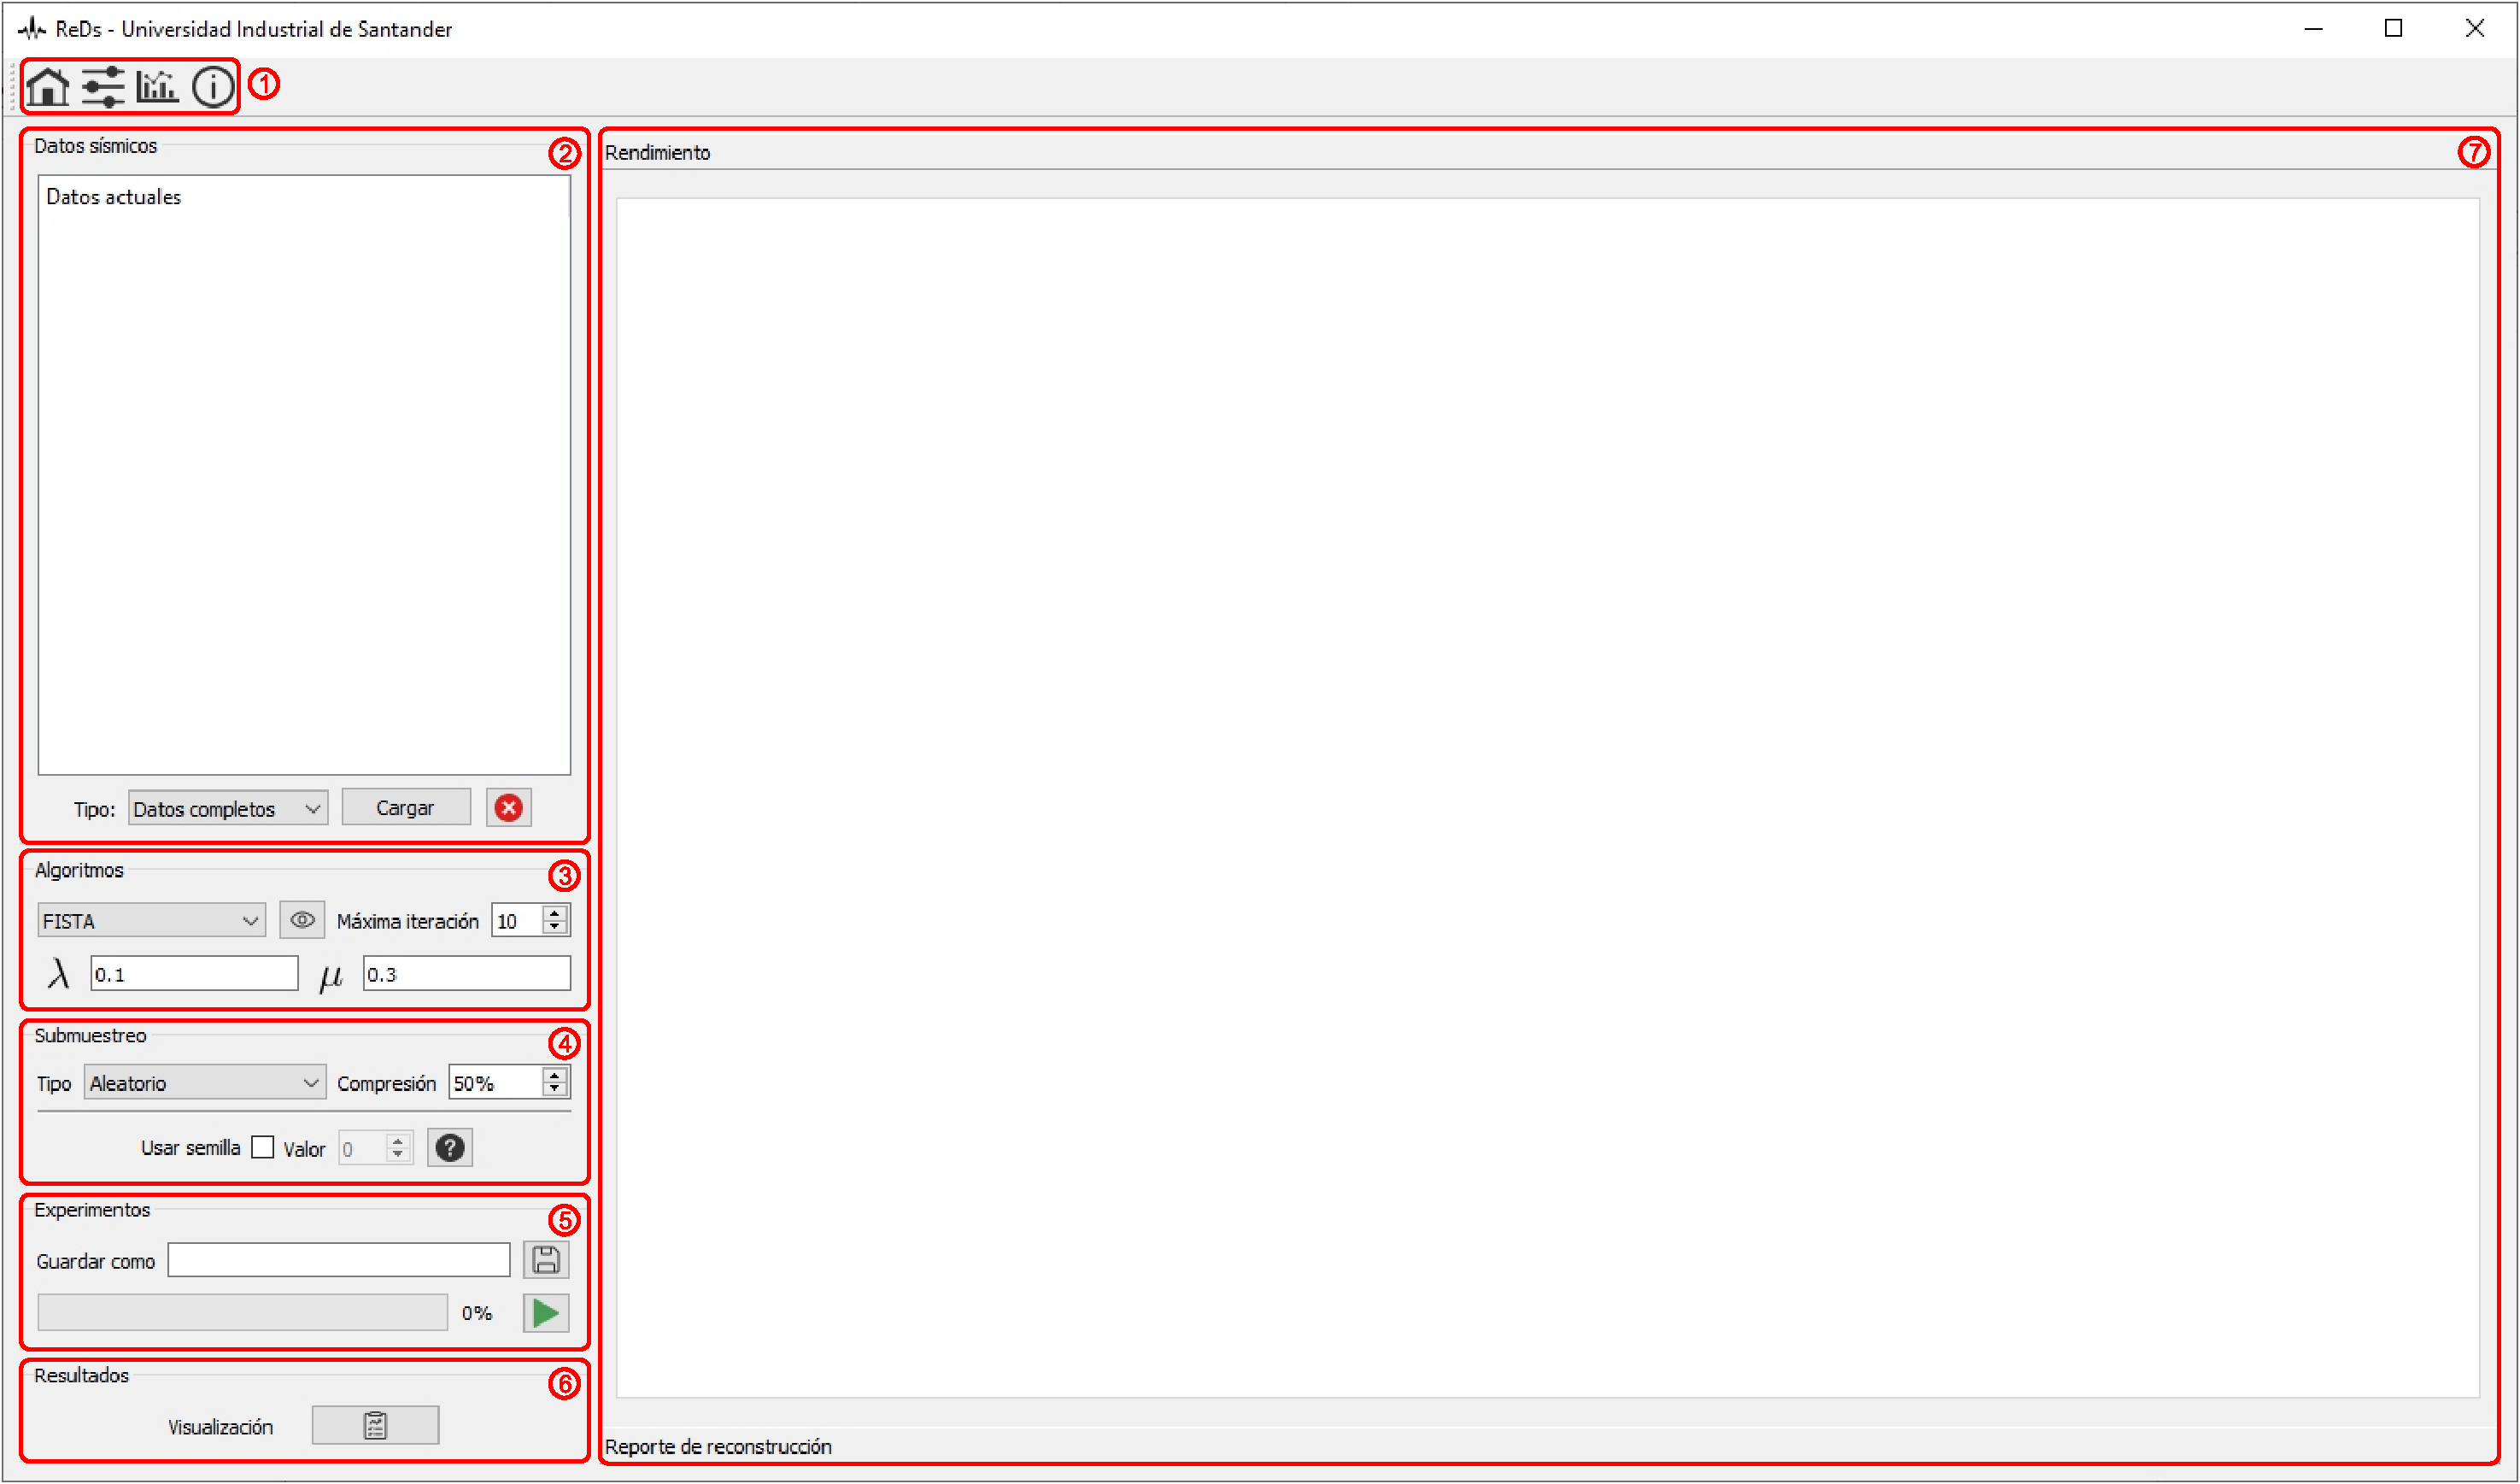
\includegraphics[width=1\linewidth]{figures/vision_v2}
	\captionof{figure}{Secciones de la interfaz general del modo Reds - RR.}
	
\end{Figure}



El menú principal permite realizar experimentos con los datos sísmicos siguiendo el orden que se observa en la figura \ref{fig:vision}. A continuación se muestra paso a paso el funcionamiento de cada uno los paneles, desde la lectura de datos sísmicos hasta la visualización y guardado de resultados.

\subsection{Políticas de diseño}

El panel de lectura de datos \circled{2}, situado al extremo izquierdo superior en la figura \ref{fig:vision}, muestra los nombres de los datos sísmicos que el usuario haya cargado en la aplicación para realizar diversas pruebas.\\

\textbf{Leyendo un dato sísmico} 

\begin{multicols}{2}
	
	\begin{Figure}
		\centering
		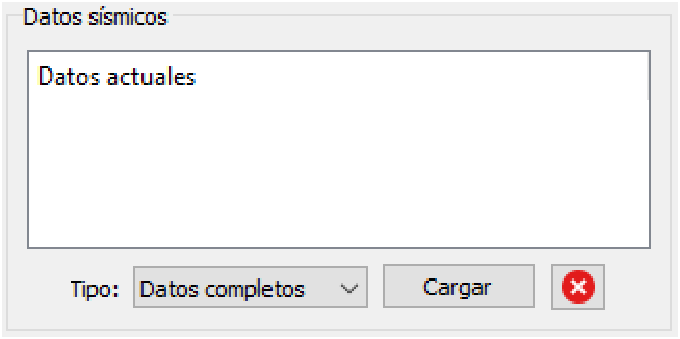
\includegraphics[width=.9\linewidth]{data-lecture-1.pdf}
		\captionof{figure}{Cargando un dato sísmico.}
		
	\end{Figure}
	
	Para leer un dato sísmico, se pulsa la opción \emph{Cargar} en el panel \circled{2}, como se observa en la figura \ref{fig:data_lecture_1}. Inmediatamente se abrirá la ventana \textit{Abrir dato sísmico}, como se observa en la figura \ref{fig:data_lecture_2}, donde el usuario podrá seleccionar un dato sísmico. Para este ejemplo cargaremos \emph{data.npy}.
	La aplicación ReDs reconoce las extensiones \emph{.npy} y \emph{.mat} para cargar datos sísmicos.
	
\end{multicols}

Existen dos tipos de datos sísmicos que pueden ser cargados desde ReDs - RR: \textit{Datos Completos} y \textit{Datos Incompletos}. El tipo de dato a ser cargado puede ser seleccionado desde la lista desplegable en la Figura \ref{fig:data_lecture_1}.

\begin{Figure}
	\centering
	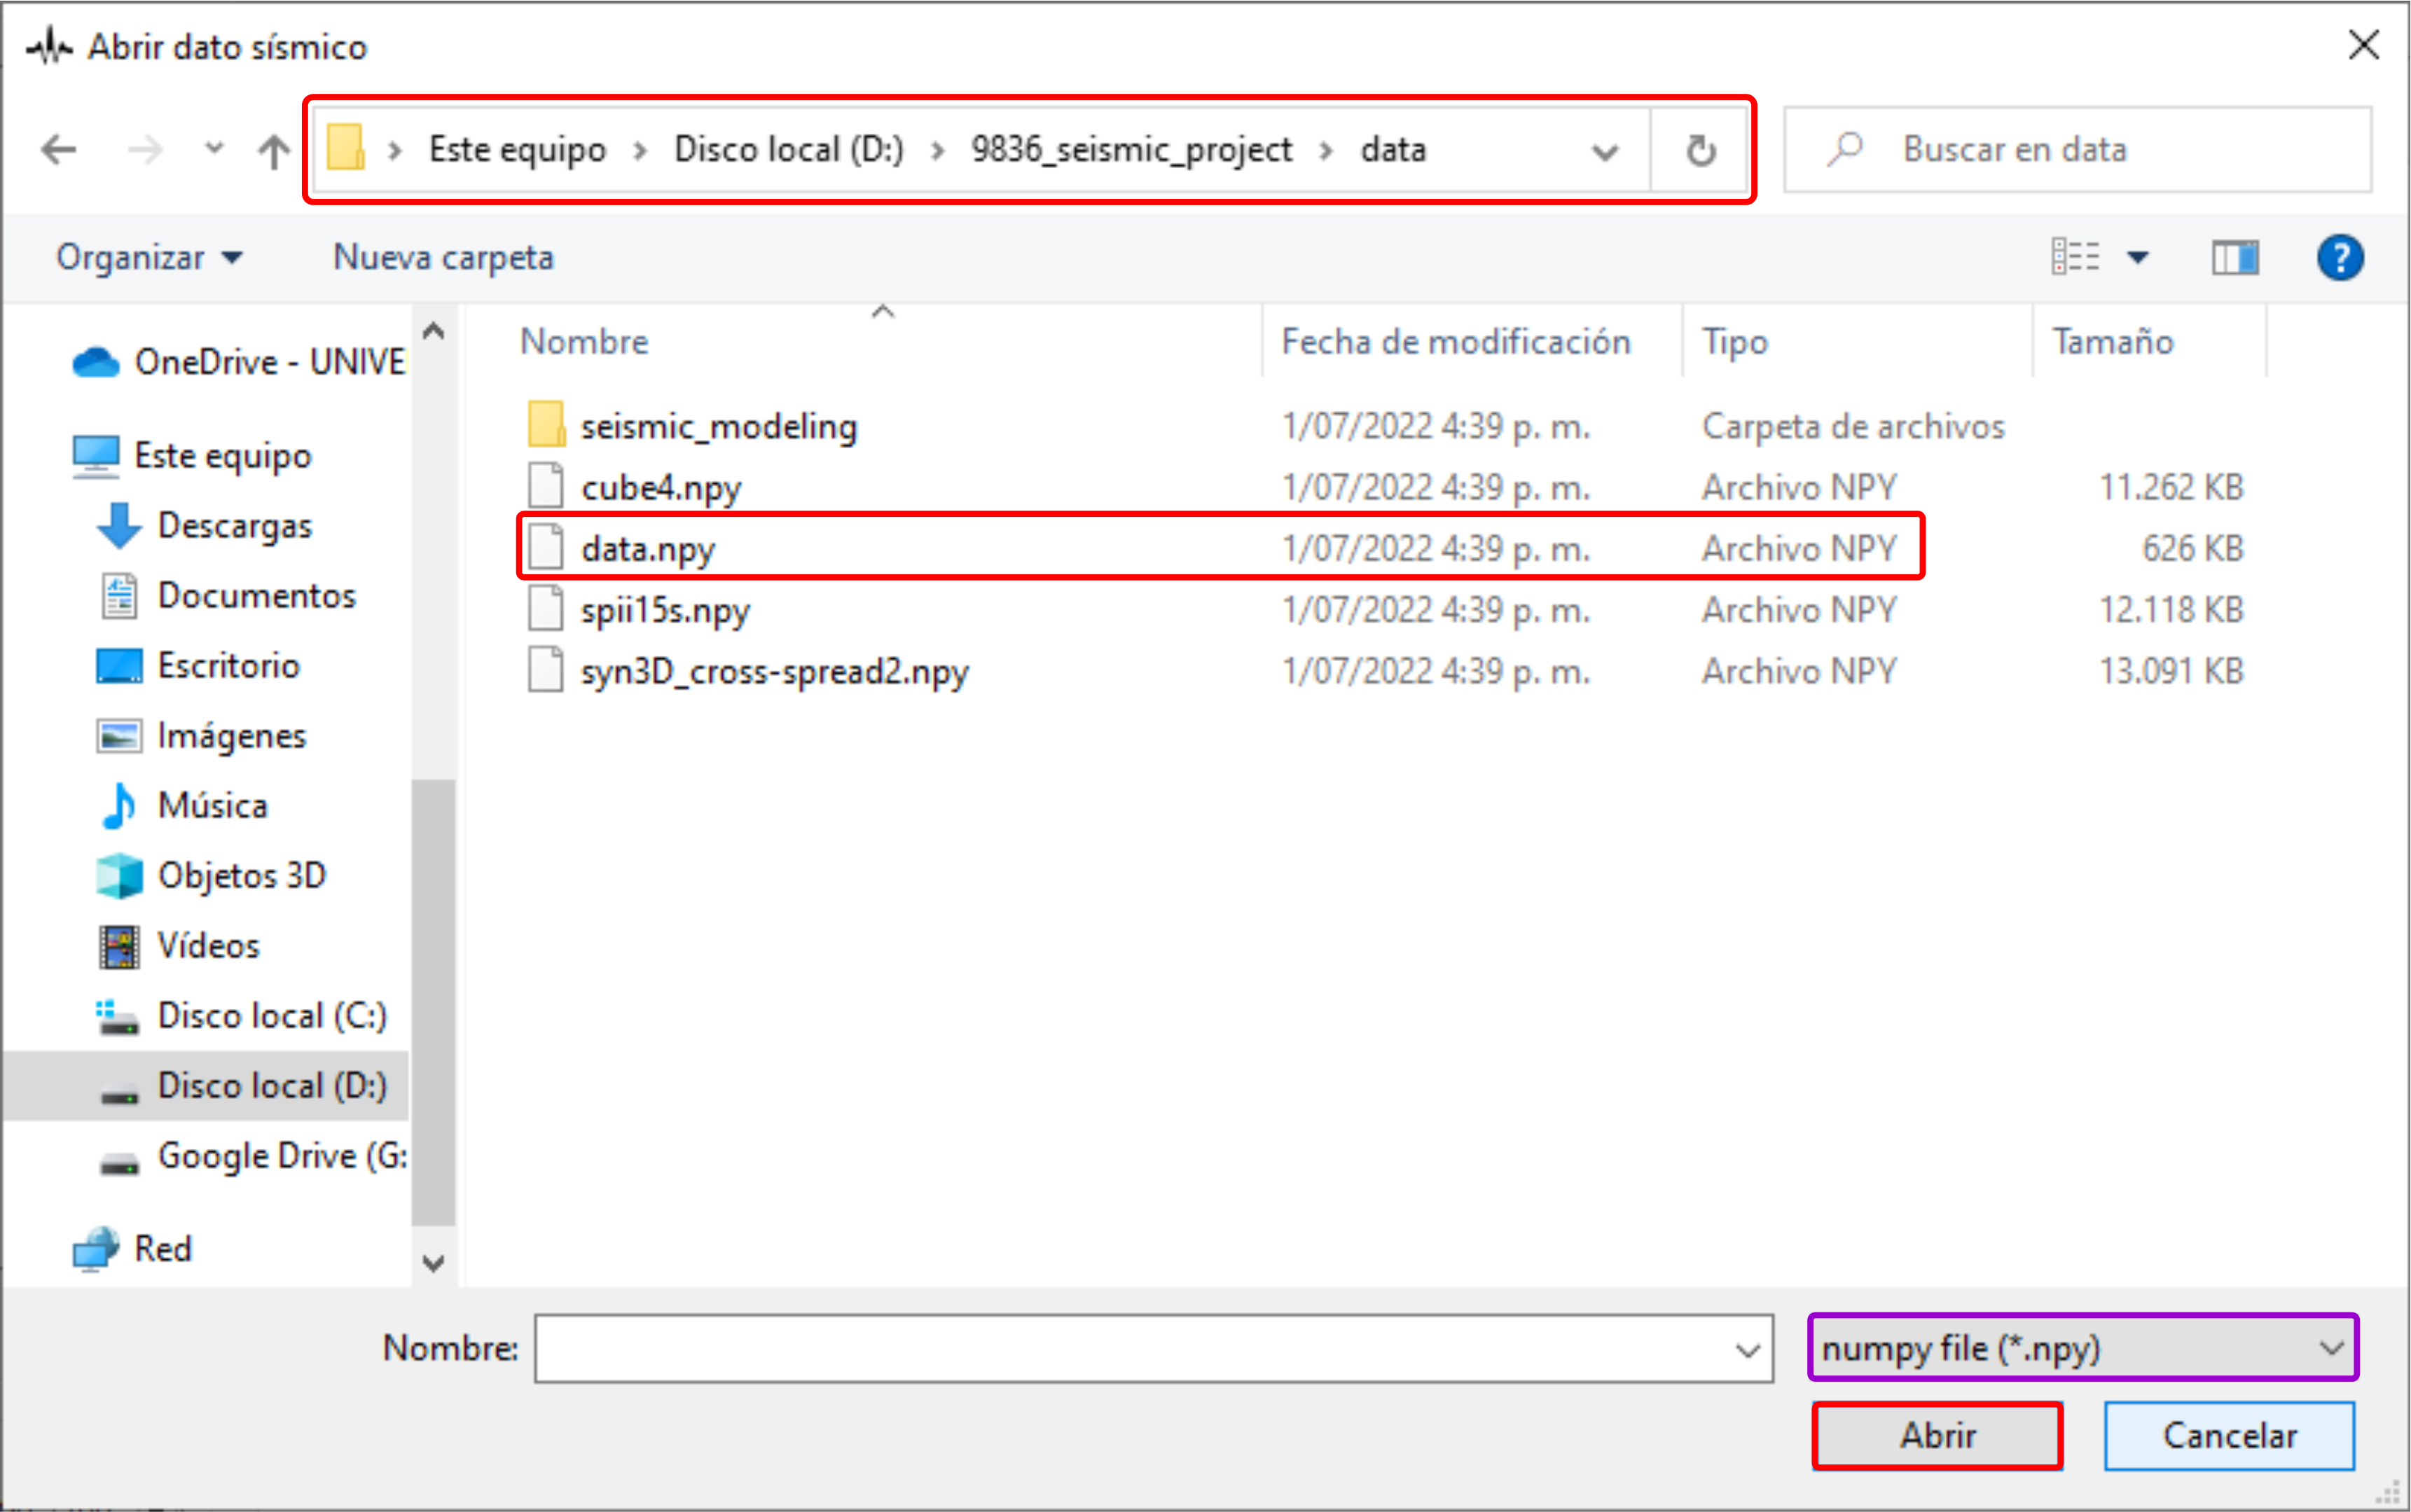
\includegraphics[width=1\linewidth]{data-lecture-2.png}
	\captionof{figure}{Ventana de selección de dato sísmico.}
	
\end{Figure}

\begin{multicols}{2}
	
	Una vez seleccionado el dato sísmico, se debe pulsar en la opción \emph{Abrir}. Se podrá observar entonces en \circled{2} el dato sísmico cargado, como se muestra en la figura . Aquí los datos se observan siguiendo la siguiente estructura: \circled{I} representa al directorio padre y \circled{II} es el dato sísmico cargado hijo del directorio padre.
	
	\begin{Figure}
		\centering
		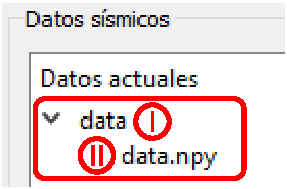
\includegraphics[width=0.6\linewidth]{data-lecture-3.pdf}
		\captionof{figure}{Panel con un dato sísmico cargado.}
		
	\end{Figure}
	
\end{multicols}

\subsection{Diagramas UML}

Los algoritmos disponibles en la aplicación son \emph{FISTA}, \emph{GAP}, \emph{TwIST} y \emph{ADMM}, tal como se observa en el panel \circled{3}, en el extremo izquierdo de la figura \ref{fig:vision}. En este panel se pueden observar las opciones de configuración de parámetros según el algoritmo seleccionado, incluyendo la cantidad máxima de iteraciones a realizar. 

\begin{figure}[!ht]
	\centering
	\begin{subfigure}[b]{0.47\textwidth}
		\centering
		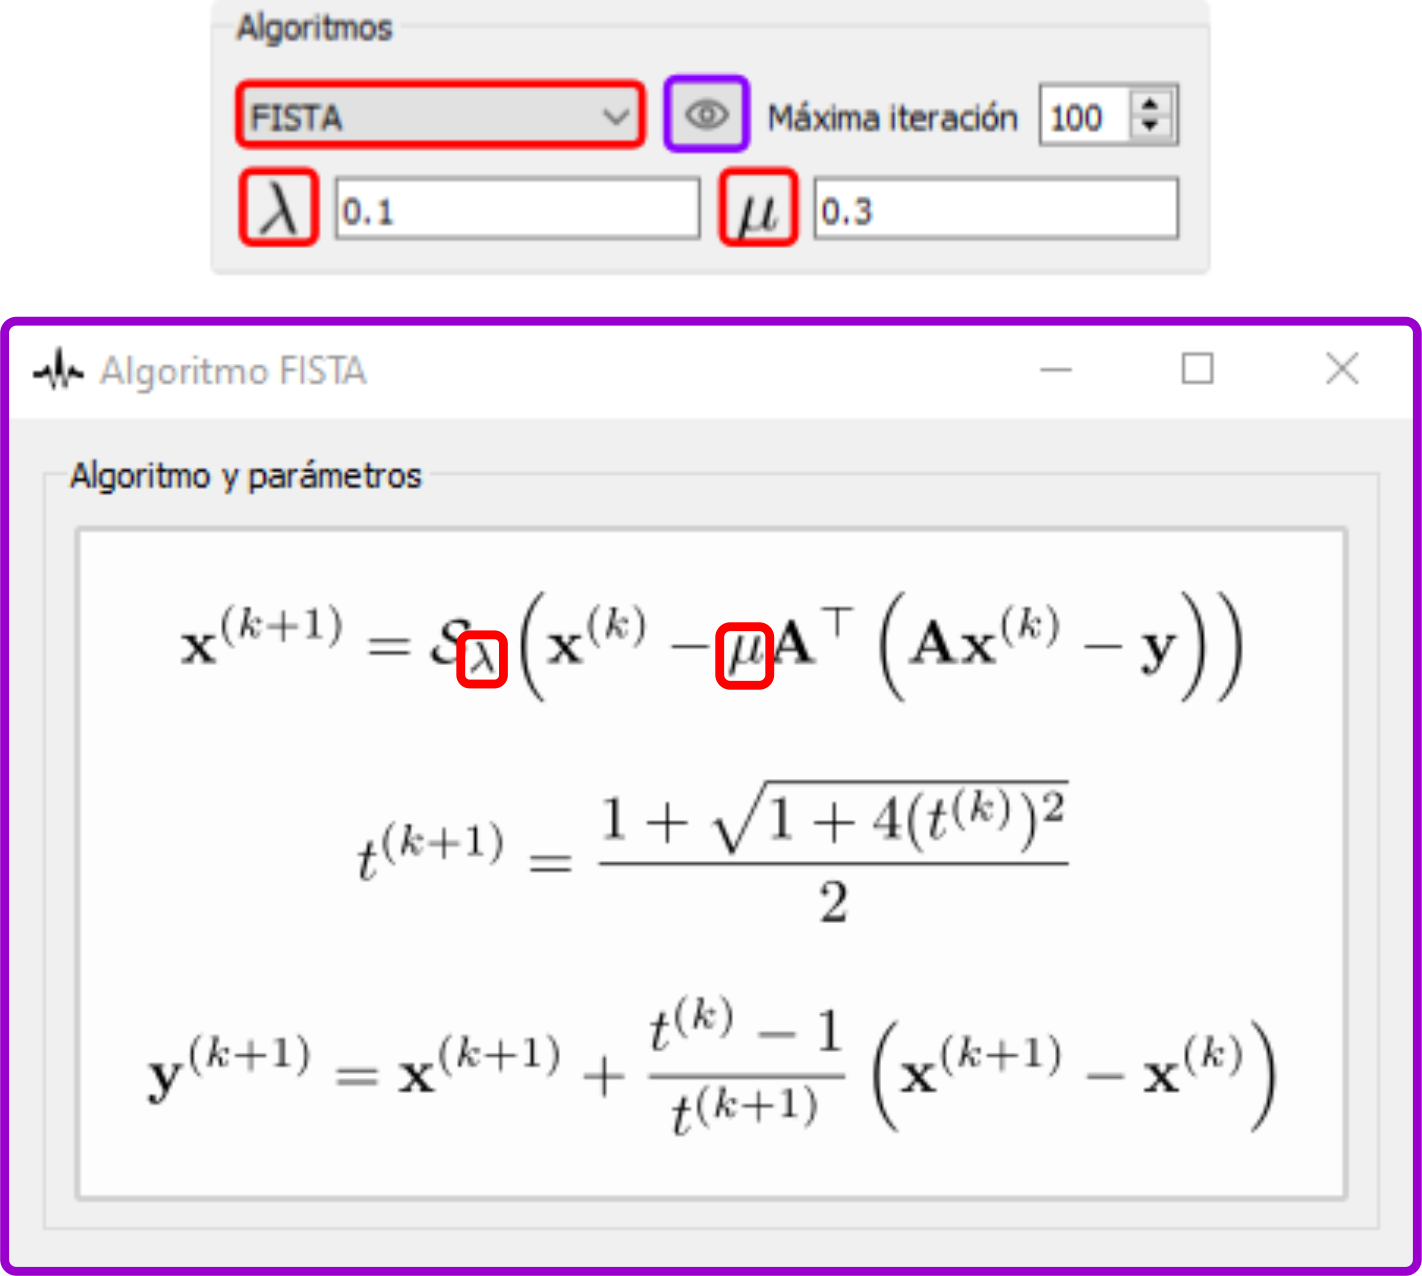
\includegraphics[width=\textwidth]{algorithm-fista.png}
		\caption{FISTA}
		
	\end{subfigure}
	\hfill
	\begin{subfigure}[b]{0.47\textwidth}
		\centering
		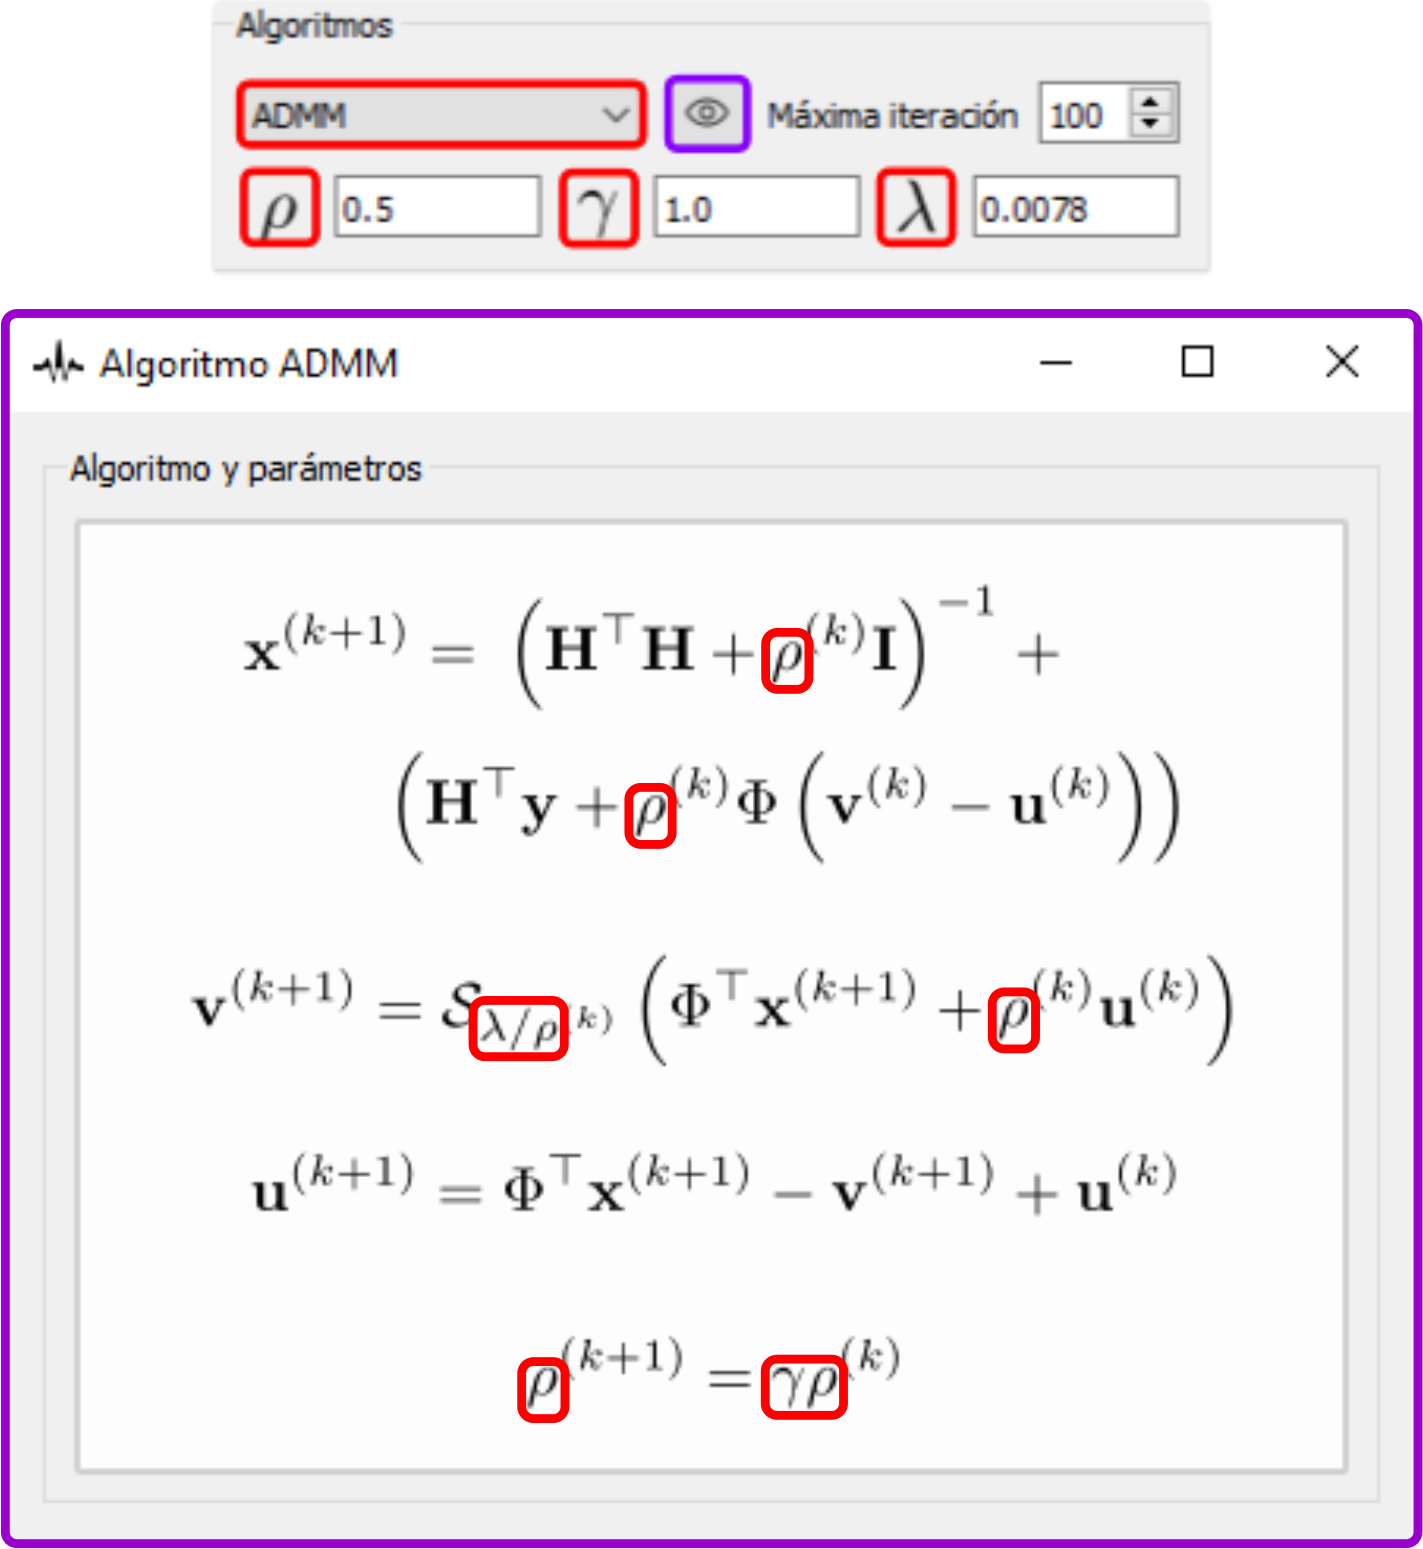
\includegraphics[width=\textwidth]{algorithm-admm.png}
		\caption{ADMM}
		
	\end{subfigure}
	\begin{subfigure}[b]{0.47\textwidth}
		\centering
		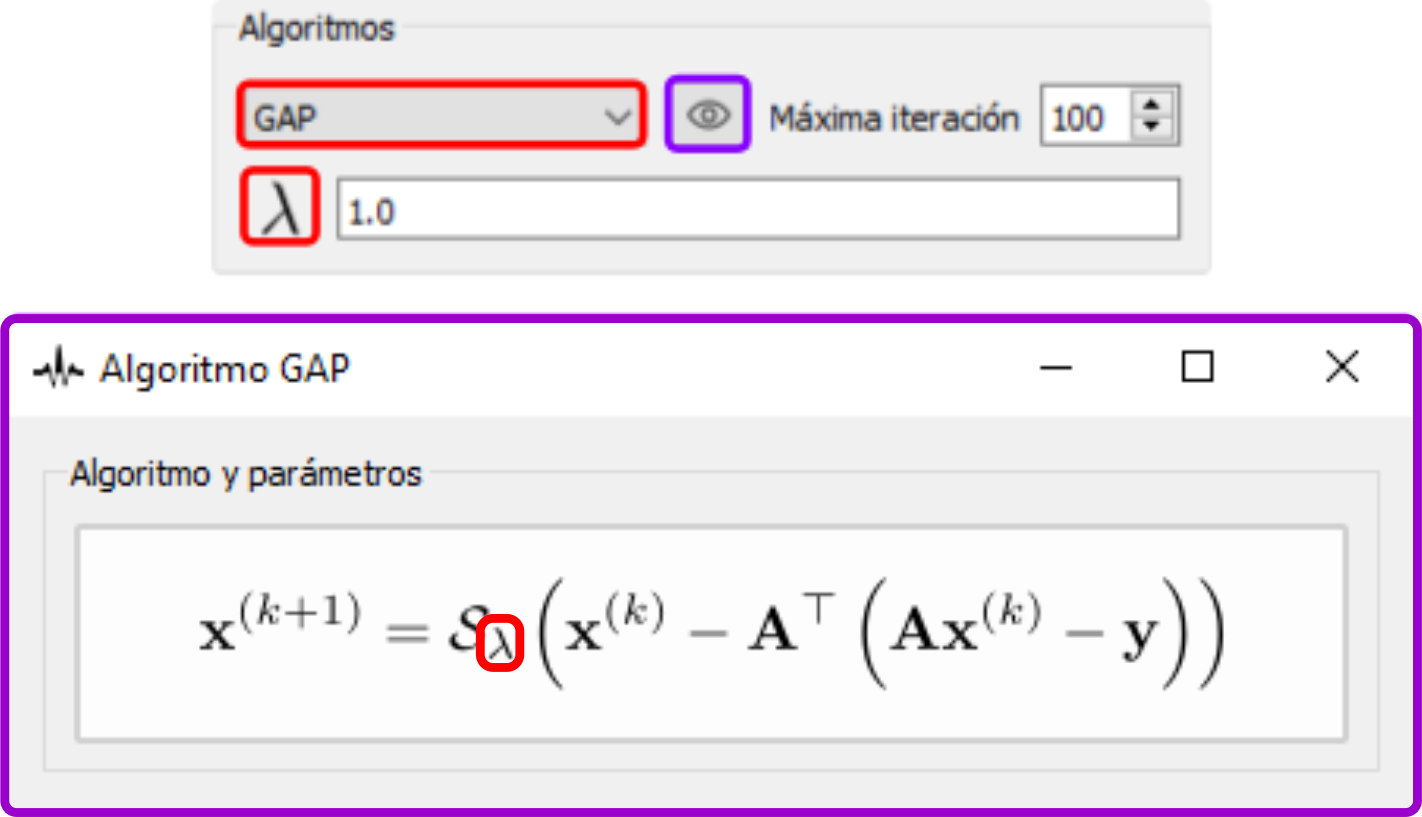
\includegraphics[width=\textwidth]{algorithm-gap.png}
		\caption{GAP}

	\end{subfigure}
	\hfill
	\begin{subfigure}[b]{0.47\textwidth}
		\centering
		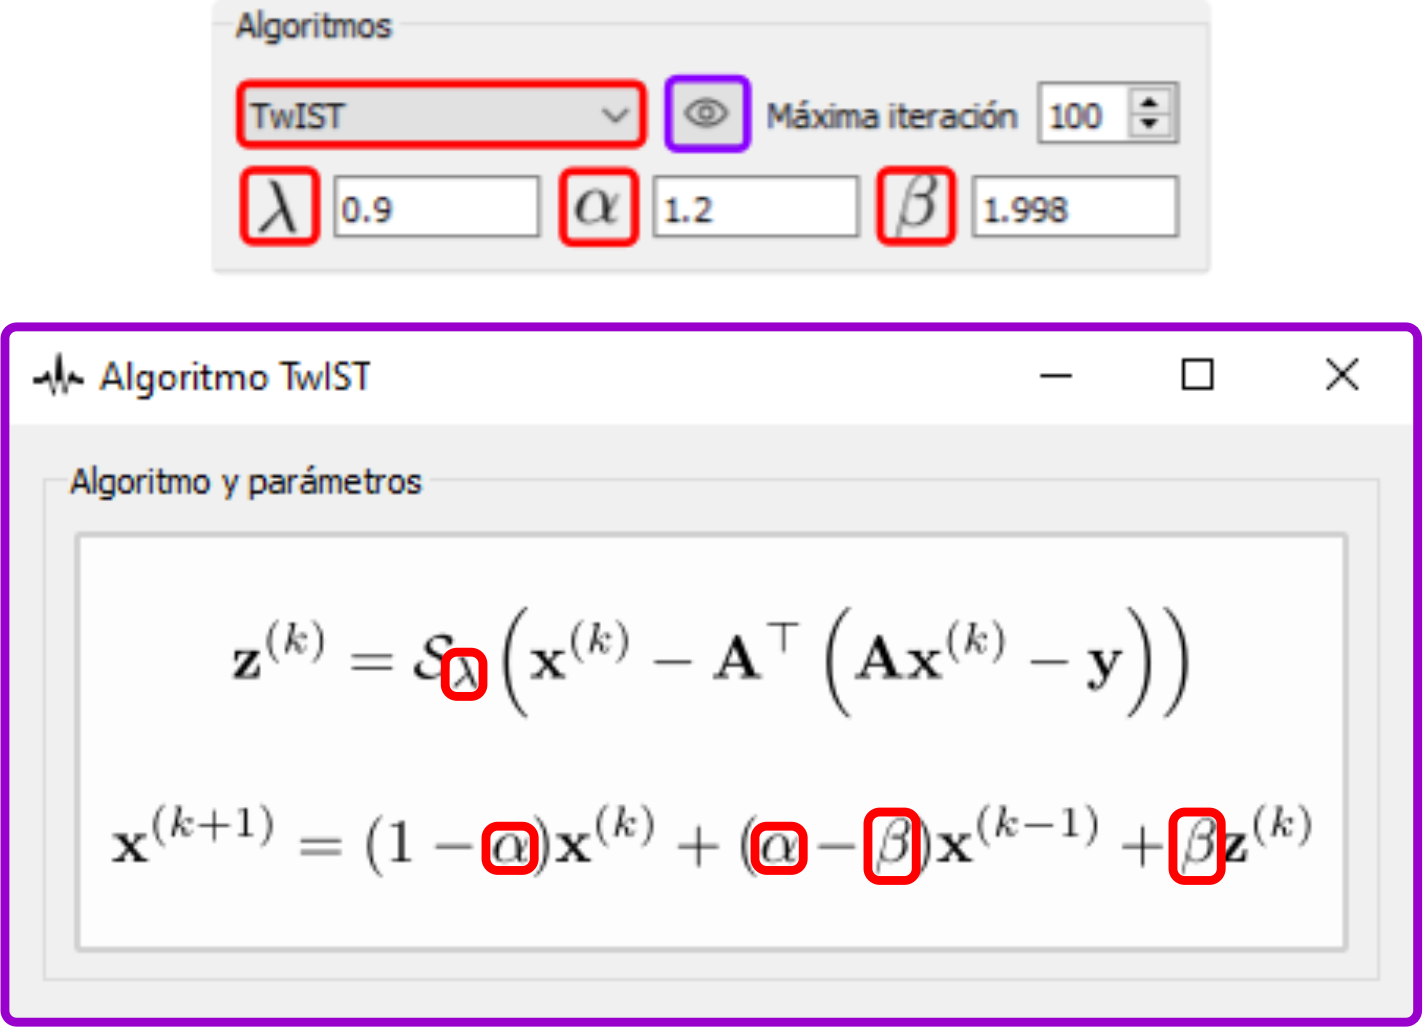
\includegraphics[width=\textwidth]{algorithm-twist.png}
		\caption{TwIST}

	\end{subfigure}
	\caption{Algoritmos disponibles y sus respectivos parámetros.}

\end{figure}

Adicionalmente, el botón\hspace{0.5mm} \faEye \hspace{0.5mm} permite visualizar los diferentes algoritmos con sus correspondientes parámetros, como se observa en la figura \ref{fig:algorithms}. Cada uno de los algoritmos disponibles cuenta con una colección propia de parámetros, los cuales el pueden ser configurados por el usuario según lo desee.

\subsubsection{Diagramas de casos de uso}

Debido a que hay varias formas de recuperar una traza a partir de las medidas recolectadas previamente, el panel de submuestreo \circled{4} permite configurar cuál tipo de submuestreo se desea realizar al dato sísmico, a manera de simulación. Todos los tipos de submuestreo, excepto el de tipo lista, comparten el mismo nivel de compresión que el usuario desee asignar. Por otra parte, al cargar datos incompletos el panel de submuestreo se deshabilita.

A continuación se presentan los tipos de submuestreo a aplicar en ReDs:\\

\underline{\textbf{Submuestreo Aleatorio}}

\begin{multicols}{2}
	\begin{Figure}
		\centering
		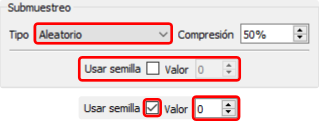
\includegraphics[width=0.8\linewidth]{subsampling-random.png}
		\captionof{figure}{Submuestreo aleatorio.}
		
	\end{Figure}
	
	Aplica un submuestreo aleatorio a las trazas sísmicas de acuerdo al nivel de compresión. Al habilitar la semilla, se puede establecer el mismo submuestreo para todas las veces que se ejecute un experimento, como se observa en la figura \ref{fig:subsampling_random}.
	
\end{multicols}

\underline{\textbf{Submuestreo Uniforme}}

\begin{multicols}{2}
	
	Aplica un submuestreo uniforme a las trazas sísmicas de acuerdo al nivel de compresión, como se observa en la figura
	
	\begin{Figure}
		\centering
		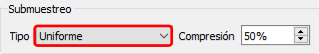
\includegraphics[width=0.8\linewidth]{subsampling-uniform.png}
		\captionof{figure}{Submuestreo uniforme.}
		
	\end{Figure}
	
\end{multicols}

\underline{\textbf{Submuestreo Jitter}}

\begin{multicols}{2}
	
	\begin{Figure}
		\centering
		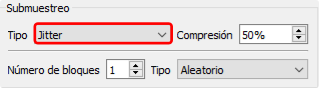
\includegraphics[width=0.8\linewidth]{subsampling-jitter.png}
		\captionof{figure}{Submuestreo jitter.}
		
	\end{Figure}
	
	Aplica un submuestreo aleatorio o uniforme de acuerdo a la cantidad de bloques ingresados por el usuario a las trazas sísmicas de acuerdo al nivel de compresión, como se observa en la figura \ref{fig:subsampling_jitter}.
	
\end{multicols}

\underline{\textbf{Submuestreo Lista}}

\begin{multicols}{2}
	
	Aplica un submuestreo de tipo lista donde las trazas a remover son ingresados por el usuario, como se observa en la figura . Para este tipo de submuestreo es necesario validar que el usuario ingrese los datos con un formato lógico y especifico.
	
	\begin{Figure}
		\vspace{5mm}
		\centering
		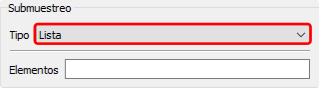
\includegraphics[width=0.8\linewidth]{subsampling-list.png}
		\captionof{figure}{Submuestreo de tipo lista.}

	\end{Figure}
	
\end{multicols}

Las condiciones son las siguientes:

\begin{multicols}{2}
	
	\begin{Figure}
		\vspace{5mm}
		\centering
		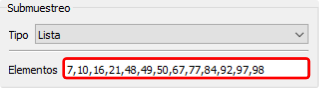
\includegraphics[width=1\linewidth]{subsampling-list-1.png}
		\captionof{figure}{Ejemplo de submuestreo de tipo lista.}
		
	\end{Figure}
	
	\begin{itemize}
		\setlength\itemsep{0em}
		\item La secuencia debe ser $x_1,x_2,x_n$, tal que $x_i \in \mathbb{Z}^+$ representa los índices de las trazas a resolver, donde entre cada $x_i$ no deben haber espacios y estar separados por números, como se observa en la figura \ref{fig:subsampling_list_1}.
		\item Cada $x_i$ debe cumplir $0 \leq x_i \leq N$, donde $N$ es la cantidad máxima lineas de receptores que contiene un \emph{shot}.
		\item Deben haber mínimo siete $x_i$ distintos.
	\end{itemize}
	
\end{multicols}

\subsubsection{Diagramas de casos de Secuencias}


Una vez ya se ha cargado un dato sísmico, seleccionado el algoritmo, ajustado sus parámetros y configurado el tipo de submuestreo, entonces se podrá realizar un experimento. El panel \circled{5}, en el extremo izquierdo de la figura \ref{fig:vision}, permite controlar el progreso de la ejecución del experimento a realizar.
\newpage
\subsubsection*{Realizando un experimento}

\begin{multicols}{2}
	
	Para iniciar un nuevo experimento se debe pulsar el botón \hspace{0.5mm} \faSave \hspace{0.5mm} que se observa en la figura \ref{fig:experiment_1}. Aquí el usuario seleccionará el directorio donde desee que los resultados de su experimento sean guardados, como se observa en la figura 
	
	\begin{Figure}
		\vspace{5mm}
		\centering
		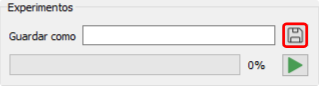
\includegraphics[width=0.8\linewidth]{experiment-1.png}
		\captionof{figure}{Panel de experimentos.}

	\end{Figure}
	
\end{multicols}

\begin{Figure}
	\centering
	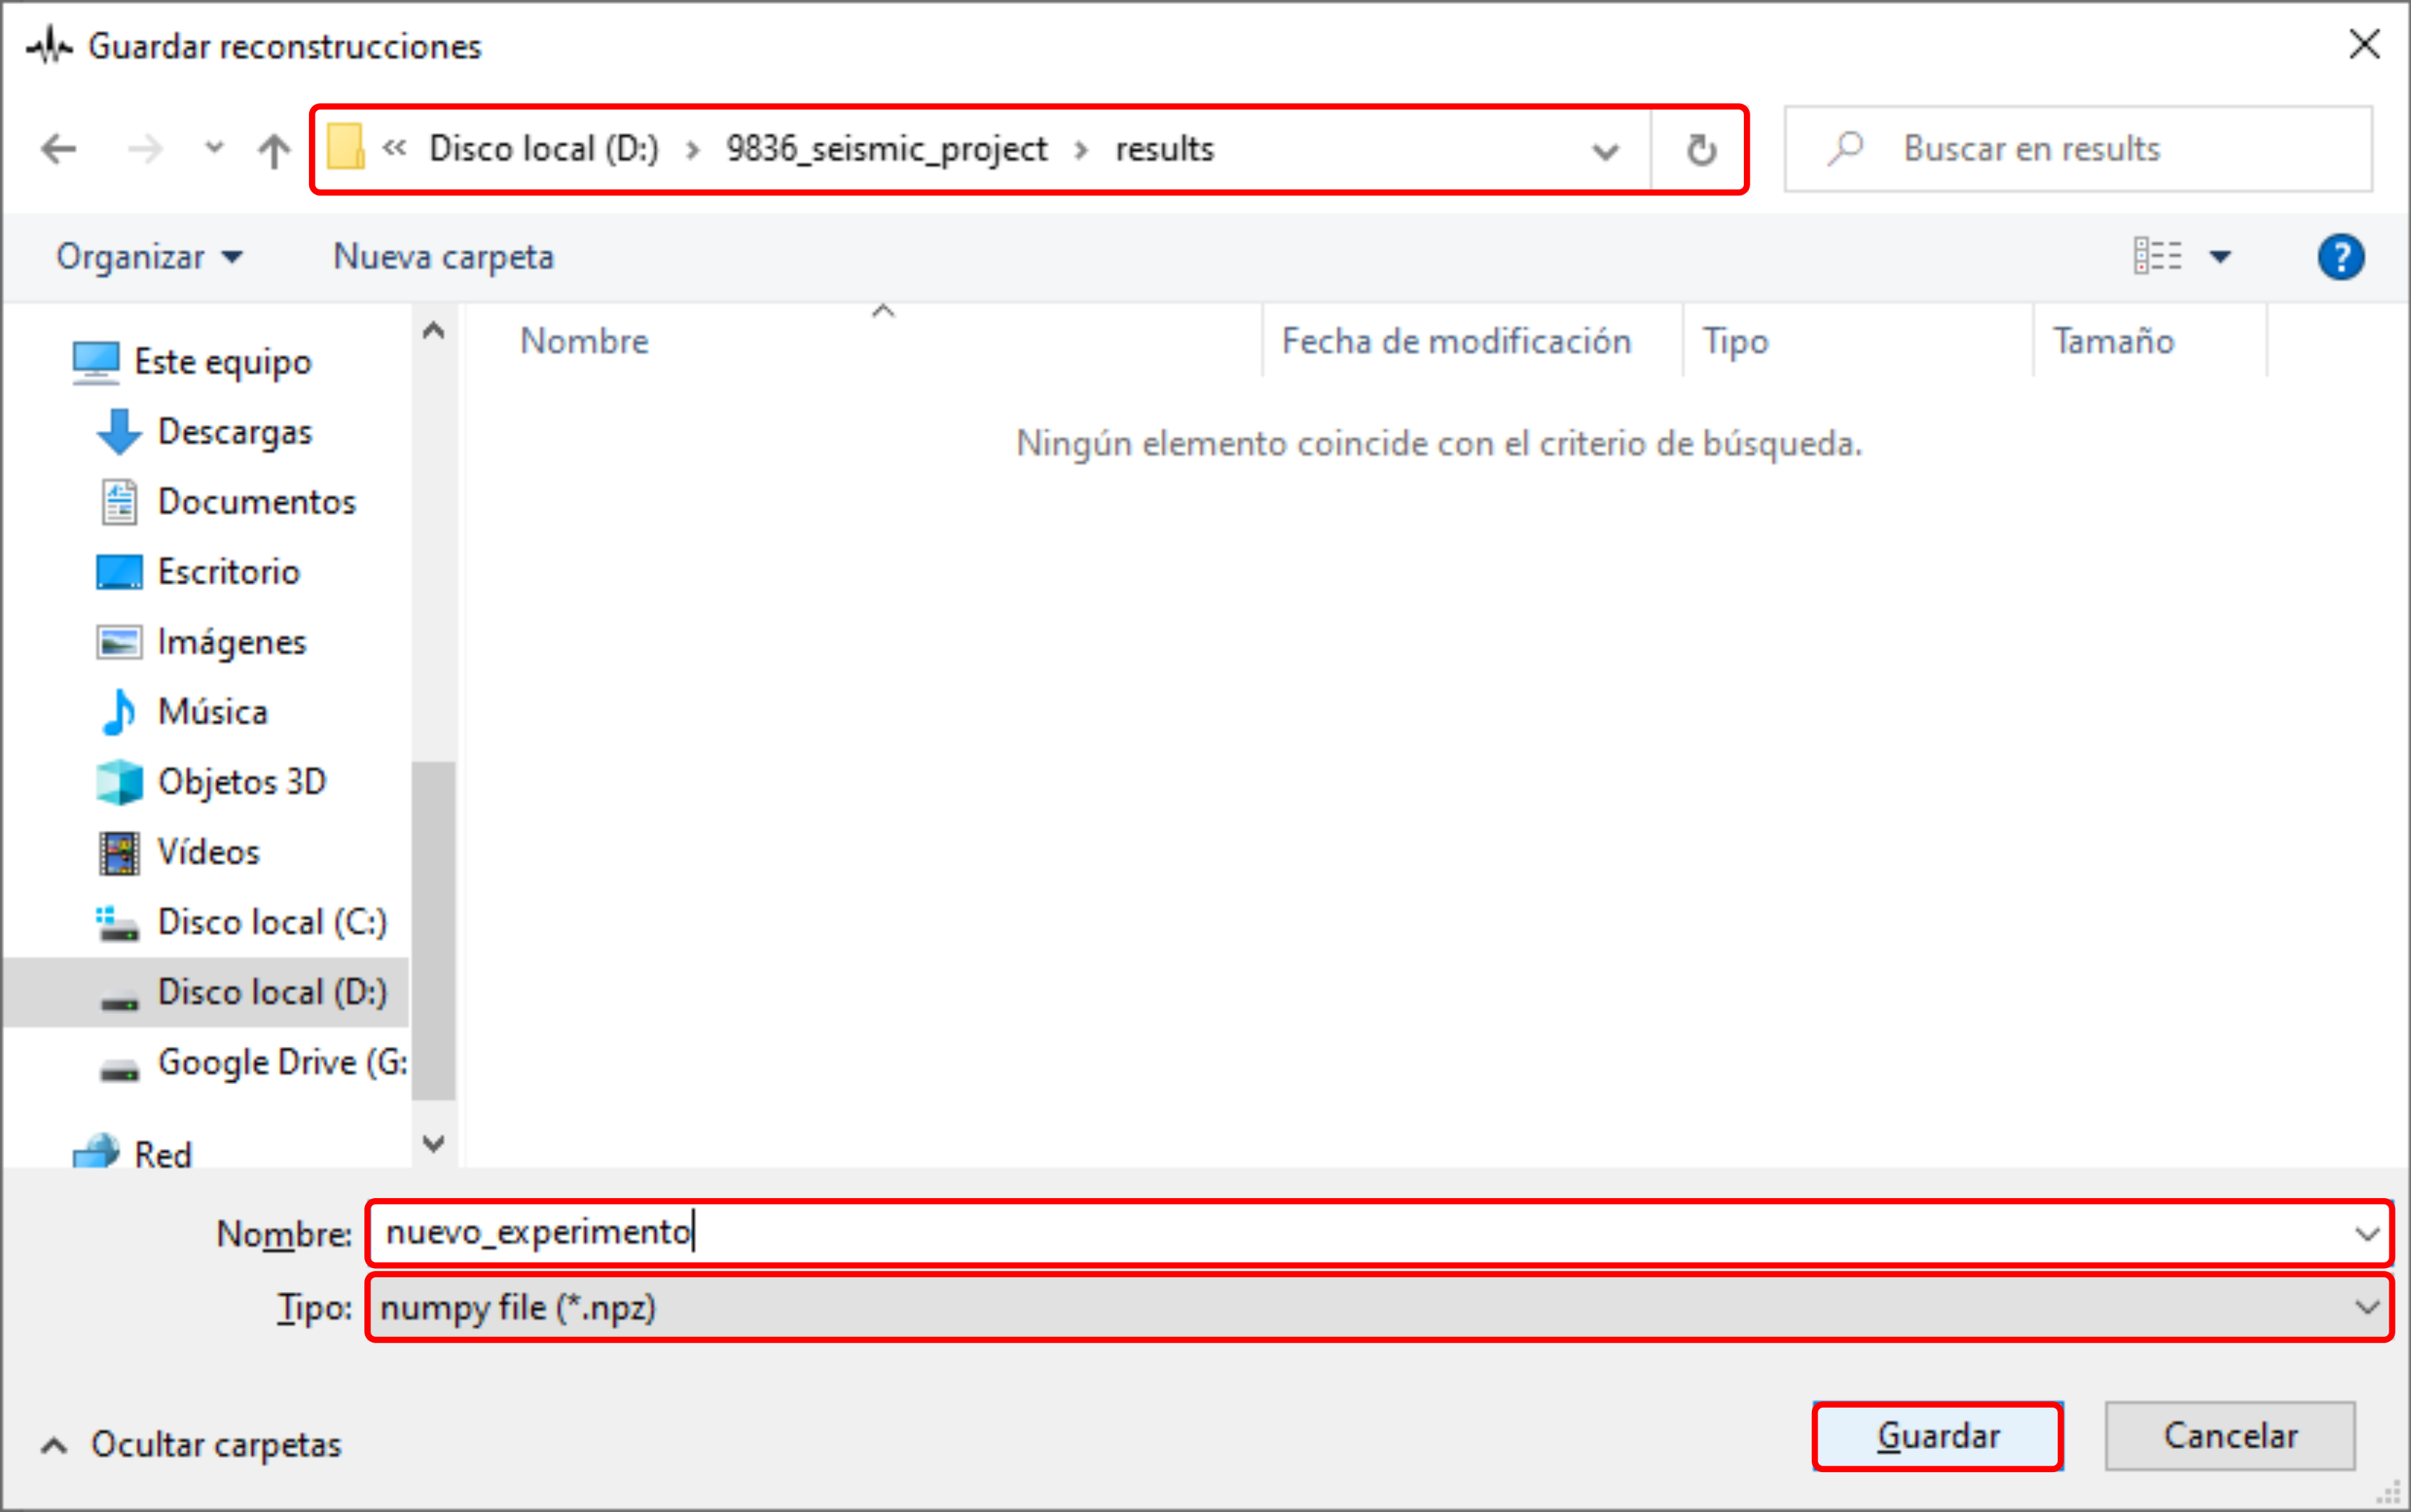
\includegraphics[width=1\linewidth]{experiment-2.png}
	\captionof{figure}{Ventana de guardado de resultados.}

\end{Figure}

Es necesario asignar un nombre al experimento para poder guardarlo. En este ejemplo usaremos \emph{nuevo\_experimento} como nombre del archivo de salida, con la extensión \emph{.npz}. Finalmente, presionamos el botón \emph{Guardar}.

\begin{multicols}{2}
	
	\begin{Figure}
		\centering
		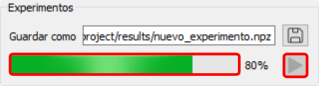
\includegraphics[width=0.7\linewidth]{experiment-4.png}
		\captionof{figure}{Ejecución de un experimento en tiempo real.}

	\end{Figure}
	
	Para correr el experimento se debe pulsar en el botón \hspace{0.5mm} \faPlay \hspace{0.5mm}. En la barra de progreso, a la izquierda de dicho botón, se podrá el progreso del actual experimento, como se observa en la figura \ref{fig:experiment_4}.
	
\end{multicols}

\subsubsection{Diagramas de Componentes}

Los resultados de todos los experimentos se pueden observar en el panel \circled{7}, en el extremo derecho de la figura \ref{fig:vision}. En este panel se encuentran dos tipos de visualización: la visualización del rendimiento (iteraciones vs. error/psnr) y visualización de la reconstrucción, como se observa en la figura \ref{fig:main_result_1}.

\begin{multicols}{2}
	
	Como se mencionó en la sección \ref{sec:experiment}, para los experimentos que sean ejecutados se podrá ver tanto el rendimiento como la reconstrucción de las trazas en tiempo real. A continuación se detallará que es lo que se observa exactamente en cada una de estos subpaneles.
	
	\begin{Figure}
		%\vspace{1cm}
		\centering
		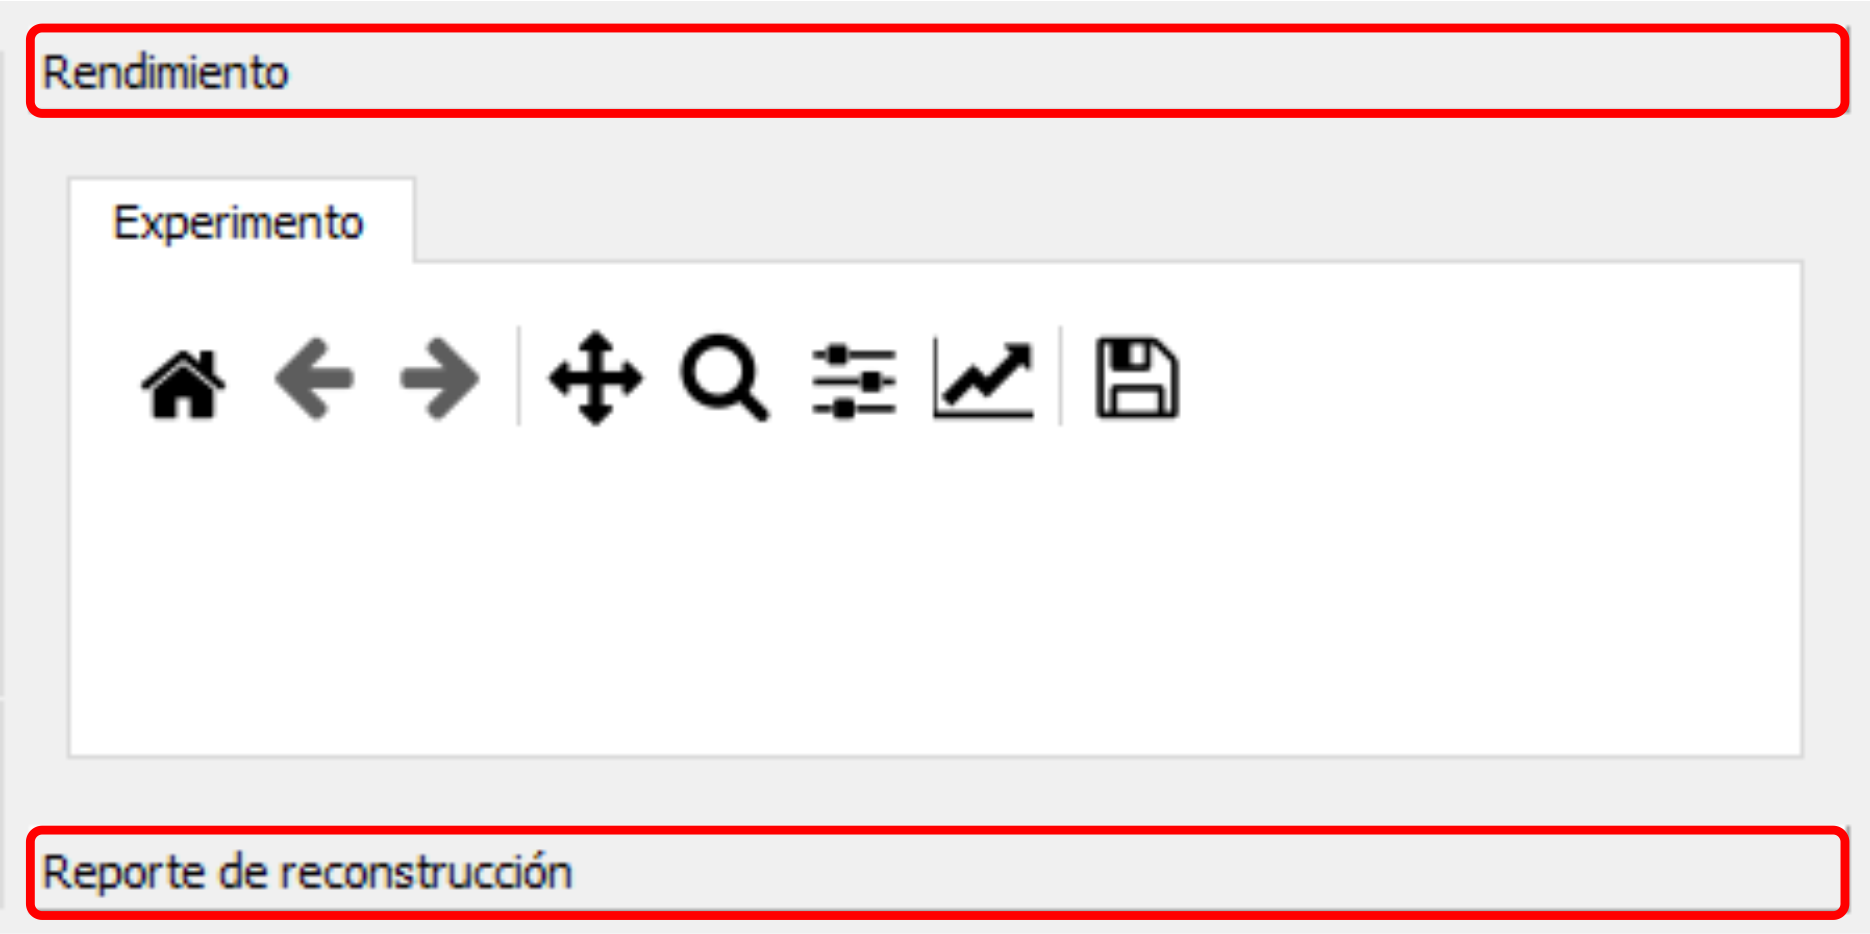
\includegraphics[width=0.7\linewidth]{main-result-1.png}
		\captionof{figure}{Panel de resultados.}
		
	\end{Figure}
	
\end{multicols}

\subsubsection{Diagramas de Clases}
\newpage
\end{document}